% ============================================================================
% Paper 2: What a passive power meter can certify about training
%
% Structure follows notes/plans/plan-for-paper-2.md §7 (provisional outline).
% ICML 2026 two-column format, [preprint] mode for arXiv (matches the sibling
% paper, tomkimpson/power-to-flops).
% ============================================================================

\documentclass{article}

\usepackage{microtype}      % microtypography
\usepackage{graphicx}
\usepackage{booktabs}       % professional-quality tables
% Every figure is regenerated by a script in ../scripts/ (see ../README.md).
\graphicspath{{../figures/}}

% hyperref makes hyperlinks in the resulting PDF. It must be loaded before
% icml2026; if a build breaks on a page-spanning link, swap to
% \usepackage[nohyperref]{icml2026} below and drop this line.
\usepackage{hyperref}

% Attempt to make hyperref and algorithmic work together better:
\newcommand{\theHalgorithm}{\arabic{algorithm}}

% [preprint] shows authors and drops the review-mode footer — arXiv version.
% Swap to plain \usepackage{icml2026} for a blind submission, or
% \usepackage[accepted]{icml2026} for camera-ready.
\usepackage[preprint]{icml2026}

\usepackage{amsmath}
\usepackage{amssymb}        % math symbols
\usepackage{mathtools}
\usepackage{amsthm}         % theorem environments (identifiability results)

\usepackage[capitalize,noabbrev]{cleveref}  % smart cross-referencing
\usepackage{aliascnt} % lets 'assumption' share the theorem counter yet be named "Assumption" by cleveref

%%%%%%%%%%%%%%%%%%%%%%%%%%%%%%%%
% THEOREMS (for the identifiability results, plan §10 Q2)
%%%%%%%%%%%%%%%%%%%%%%%%%%%%%%%%
% Every environment shares the theorem counter so numbering runs in a single
% sequence. Plain [theorem] sharing would make cleveref call them all
% "Theorem"; aliascnt gives each its own counter name, so \cref renders
% "Proposition 3.2", "Assumption 3.8", and so on.
\newtheorem{theorem}{Theorem}[section]
\newcommand{\sharedtheorem}[3]{%
	\newaliascnt{#1}{theorem}%
	\newtheorem{#1}[#1]{#2}%
	\aliascntresetthe{#1}%
	\crefname{#1}{#2}{#3}%
	\Crefname{#1}{#2}{#3}%
}
\theoremstyle{plain}
\sharedtheorem{proposition}{Proposition}{Propositions}
\sharedtheorem{lemma}{Lemma}{Lemmas}
\sharedtheorem{corollary}{Corollary}{Corollaries}
\theoremstyle{definition}
\sharedtheorem{definition}{Definition}{Definitions}
\sharedtheorem{assumption}{Assumption}{Assumptions}
\theoremstyle{remark}
\sharedtheorem{remark}{Remark}{Remarks}

% Short form of the title for the running header:
\icmltitlerunning{What a Power Meter Can Certify About Training}

\begin{document}

\twocolumn[
  \icmltitle{What a Passive Power Meter Can Certify About AI Training}

  \begin{icmlauthorlist}
    \icmlauthor{Tom Kimpson}{unimelb}
    \icmlauthor{Mauricio Baker}{rand}
    \icmlauthor{Emlyn Graham}{tbd}
    \icmlauthor{Anjay Friedman}{rand}
    \icmlauthor{Coby Joseph}{rand}
  \end{icmlauthorlist}

  \icmlaffiliation{unimelb}{School of Mathematics and Statistics, The University of Melbourne, Parkville, VIC 3010, Australia}
  \icmlaffiliation{rand}{RAND Corporation}
  \icmlaffiliation{tbd}{Affiliation TBD} % TODO: Emlyn Graham's affiliation

  \icmlcorrespondingauthor{Tom Kimpson}{tom.kimpson@unimelb.edu.au}

  % Keywords populate the PDF metadata; they are not shown in the document.
  \icmlkeywords{AI governance, compute verification, power side channel, cyclostationary detection}

  \vskip 0.3in
]

% Creates the first-column footnote with affiliations; required even if empty.
\printAffiliationsAndNotice{}

\begin{abstract}
Compute-governance regimes that register or restrict large training runs
presuppose that a regulator can tell when training happens on monitored
hardware, and a power meter outside the prover's control is the one passive
channel available against a prover who does not cooperate. We ask what such a
meter can certify, and organise the answer as a ladder of four claims of
increasing governance relevance, each with a stated information cost and a hard
ceiling. Evidence is developed on a literature-parameterized scenario model of
datacentre AI workloads together with an explicit off-chip observation model,
against both a benign prover and an adaptive one who knows the detector. We
find that the iteration cadence of synchronous training is recoverable by a
tracked cyclostationary detector, but that the complete
tracker--resample--test pipeline admits no analytic calibration, so we report
it as an effective score with per-trace surrogate calibration rather than as a
constant false-alarm-rate test. Our central result is the de-periodicisation
frontier, which prices hiding against measured throughput anchors and is
strongly asymmetric: a prover that varies real work per iteration hides from
every fixed-frequency test at essentially zero cost, while the best anchored
attack against the tracking class buys little hiding for a $159\%$ overhead.
Two limits are firmer than the detectors. The observation channel is itself a
condition on every claim --- a one-second-integrating, one-hertz meter defeats
all detectors on an unmodified honest workload --- and the meter certifies a
physical schedule rather than training semantics: five non-training loads,
including one that computes gradients and discards them, are classified as
training by every rule we test. Escaping that ceiling requires leaving the
passive channel for an active challenge protocol, which we specify but do not
run. Real hardware enters as a negative transport case: on a single GPU the
cadence signature is roughly $75$ times shallower than the model assumes,
which we attribute to the absence of distributed synchronisation and state as
a falsifiable prediction rather than a result.
\end{abstract}


% ============================================================================
\section{Introduction}
\label{sec:intro}
% ============================================================================

Compute governance proposals call for evaluations, audits, and the
registration or prohibition of training runs above specified compute
thresholds
\citep{shavit2023chinchilla,sastry2024computing,baker2025verifying,heim2024thresholds};
U.S.~Executive Order 14110 briefly operationalised one such threshold,
requiring the reporting of training runs above $10^{26}$ FLOP
\citep{whitehouse2023eo14110}. Every such scheme presupposes that a regulator
can tell when training occurs on monitored hardware. Detection from
prover-owned telemetry is feasible but conditional on tamper-resistant read
paths that do not yet exist
\citep{rahman2026telemetry,ogara2025hardware}; active challenge-response
protocols remove the trust anchor but require the prover's participation
\citep{monfared2026timing}. A power meter outside the prover's control is the
one passive channel a verifier can read today against an uncooperative
prover. This paper asks, as a theory-and-methods question: what can such a
meter certify, with what methods, at what cost in verifier information, and
against an adversary who knows the detector?

Our answer is that a passive external power trace can provide calibrated
structural evidence, and conditional evidence of efficient
iteration-structured training, but not universal semantic identification. An
adaptive prover can attack the exposed cadence, and the empirical question is
what detection--utility frontier erasing it requires. Stronger work
verification is possible only conditionally, on additional challenge and
transcript primitives.

\paragraph{A ladder, not a detector.}
That answer is not a single yes or no, so we do not organise the paper around
a single test. We organise it as a \emph{claim ladder}
(\cref{tab:ladder}): four claims of increasing governance relevance, each
bought at a stated cost in verifier information, and each with a hard ceiling
that motivates the next. Rung~1 establishes that order-coherent power
structure is present, which is evidence rather than identification. Rung~2
converts that structure into training-likeness, at the price of committing to
an inference null; its ceiling is the semantic decoy. Rung~3 escapes both the
null and the decoy by binding the physical response to an unpredictable
challenge, at the price of the prover's cooperation; its ceiling is a
challenge-aware dummy load. Rung~4 ties the response to declared work, but
only given a transcript primitive we assume rather than build. Each rung is
the principled response to the previous rung's ceiling, and the contribution is
mapping the ladder honestly --- including where each rung stops. The ladder is
analogous in spirit to an attestation ladder in which more verifier information
permits a stronger claim at greater institutional cost, but it is a ladder of
claims and assumptions, not a quantitative bound on unidentified compute.

Within every rung we run two adversary settings: a \textbf{benign}
(non-adaptive) prover who runs its workload without regard to the meter, and
an \textbf{adaptive} (hiding) prover who knows the detector and reshapes its
schedule to evade it. Most of what is interesting lies in the gap between them.

\paragraph{Scope.}
We use the time-resolved power trace and exclude the integrated-energy channel:
no bounding of how much compute was performed, no energy-per-token pricing as a
verification instrument. This is a restriction on the observable, not a claim
that everything lives in the spectrum --- cyclostationary structure is expressed
spectrally, but the challenge correlation of Rung~3 is a time-domain operation
on the same trace.

\paragraph{Target population.}
We do not claim a recoverable cadence is universally necessary for training.
Some conceivable execution can be made fully aperiodic. Instead we target
efficient, synchronous, iteration-structured training that exposes a
recoverable cadence --- an expected physical signature of that regime,
especially where distributed synchronisation makes the modulation deep and
coherent. Destroying that cadence is then an adversarial action with a
measurable budget, not a counterexample to the method, and measuring that
budget is what \cref{sec:frontier} does.

\paragraph{Why theory and methods, rather than hardware.}
We do not have hardware that can test the real question. The iteration cadence
exists on a single GPU, and our measurements find the corresponding ripple at
about $0.40\%$ of board power, but a single saturated card has no
communication phase, so the modulation is shallow and easily washed out. A
single-node rig matches neither a datacentre nor the aggregate regime of the
workload model we adopt. All evidence therefore lives on a
literature-parameterized scenario model (\cref{sec:scenario}), which we are
careful not to call calibrated: a factor of roughly $75$ separates the
modulation depth that model assumes from what we measure on one A100. Real
hardware enters as a negative transport case (\cref{sec:reality}), not as a
pillar, and the prediction that distributed synchronisation deepens and coheres
the signature is stated as falsifiable rather than claimed as a result.

\paragraph{Contributions.}
\begin{enumerate}
	\setlength{\itemsep}{1pt}
	\item \textbf{The claim ladder} (\cref{tab:ladder}) as an organising frame
	for passive compute verification: four claims, their information costs, and
	their ceilings, closed out one by one in \cref{tab:closeout}.
	\item \textbf{A tracked cyclostationary detector for Rung~1}
	(\cref{sec:structural}), with a negative methodological result we report
	rather than bury: no covariance configuration calibrates the complete
	tracker--resample--test pipeline end to end, so it is not a constant
	false-alarm-rate test and we do not present it as one. It is an effective
	score with per-trace surrogate calibration, level-exact on the
	linear-stationary nulls we tested. A pre-registered bake-off
	(\cref{app:bakeoff}) makes the choice of detector an outcome, and against a
	Whittle likelihood-ratio ceiling the tracker is essentially optimal on the
	inference null while only the cyclostationary order family approaches the
	ceiling on structural confusers.
	\item \textbf{The de-periodicisation frontier} (\cref{sec:frontier}), the
	central result, priced against measured throughput anchors. Its shape is an
	asymmetry: against fixed-frequency tests a prover reaches a hiding rate of
	$0.74$ at essentially zero throughput cost by varying real work per
	iteration, whereas against the tracking class the best anchored attack
	reaches only $0.16$ at $159\%$ overhead.
	\item \textbf{A minimum meter specification} (\cref{subsec:meter_spec}):
	the observation channel is a first-class condition on every rung, and we
	locate where each detector class dies in sample rate, integration window,
	and in-band transfer function. A $1$\,s-integrating, $1$\,Hz-reporting meter
	defeats every detector on an unmodified honest workload.
	\item \textbf{Rung-2 classification with semantic falsification controls}
	(\cref{sec:classification}). Three decision rules separate training from the
	stated inference null perfectly and survive six domain shifts; but five
	non-training loads, including a decoy that computes gradients and discards
	them, all score as training. The meter certifies the physical schedule, not
	training semantics --- a ceiling no better passive detector removes.
	\item \textbf{A negative transport case} (\cref{sec:reality}): what we
	measured on real hardware, why it does not carry the distributed claim, and
	what would falsify the prediction that it should.
\end{enumerate}

Supporting these, \cref{subsec:identifiability} gives the formal counterpart of
the Rung-1 and Rung-2 ceilings: an observational-equivalence argument for why
no passive test can identify training semantics, and a covertness cost bound
showing that a prover using i.i.d.\ phase jitter to reach a target covertness
level against an exhibited verifier must pay in throughput or learning
efficiency. We are explicit about what that bound does not cover, and
\cref{sec:frontier} supplies the near-free attack that shows why the gap
matters.

\begin{table*}[t]
	\centering
	\small
	\caption{The claim ladder. Each rung answers a
	strictly more governance-relevant question at a stated cost in verifier
	information; each rung's hard ceiling motivates the next. Within each rung
	we consider a benign (non-adaptive) and an adaptive (hiding) prover.
	\Cref{tab:closeout} closes each rung out against the evidence.}
	\label{tab:ladder}
	\begin{tabular}{@{}p{2.6cm}p{4.2cm}p{3.4cm}p{4.6cm}@{}}
		\toprule
		Rung & Claim & Additional requirement & Hard ceiling \\
		\midrule
		1. Structural evidence & Order-coherent power variation exists under a
		specified structural null & External time-resolved trace only &
		Periodic physical confounds; structural-null misspecification; strong
		superposition or dilution; active power shaping; cadence moved outside
		the searched family; die-to-meter attenuation \\
		2. Conditional classification & The trace is more training-like than
		the stated inference population & A representative or explicitly
		modelled inference null & Domain shift; the semantic decoy
		(training-shaped execution without retained training) \\
		3. Active physical authentication & A load behind the meter responded
		to an unpredictable verifier challenge & Prover participation; a
		challenge-bound schedule & A challenge-aware dummy load; no semantic
		binding by power alone \\
		4. Work verification & The physical response is tied to declared
		training state transitions & A sound, fresh transcript/proof and an
		explicit binding assumption & The remote-proof / co-location gap,
		unless the assumed primitive closes it \\
		\bottomrule
	\end{tabular}
\end{table*}


% ============================================================================
\section{Related work}
\label{sec:related}
% ============================================================================

% Written from notes/discussion/st0-prior-art-audit.md (four-field prior-art
% audit). Structured by the four mature literatures the problem borrows from;
% the contribution is the question, the adversary, and the channel, not the
% detectors.
Four mature literatures own pieces of this problem. We take their tools off
the shelf; what is new here is the question (compute governance), the adversary
(a prover who knows the detector and reshapes the trace to evade it), and the
channel (a single, filtered, low-rate meter outside the prover's control). We
locate the work against each in turn, and against the closest governance-specific
detectors cited in \cref{sec:intro}.

\paragraph{Non-intrusive load monitoring.}
Inferring which devices or activities are running from a single aggregate power
meter is the founding problem of non-intrusive load monitoring
\citep{hart1992nilm}, with three decades of disaggregation
technique---edge/event detection, steady-state signatures, and state-space
models \citep{zoha2012nilm}. Certifying training from one datacenter meter is
this problem lifted from the household scale. The load-bearing difference is the
adversary: classical NILM assumes cooperative or indifferent appliances and
targets their steady-state or transient-edge signatures, whereas our load
actively hides, and the signature we exploit is a quasi-periodic,
frequency-wandering second-order structure rather than a switching event. The
power-side-channel malware detector of \citet{clark2013wattsupdoc} is the same
idea one level up in bandwidth, again without an evading adversary.

\paragraph{Spectrum sensing and low-probability-of-detection signals.}
Deciding whether a source is active, and what it is doing, from noisy
observations---explicitly against a transmitter trying to stay below the
detection floor---is the subject of spectrum sensing in cognitive radio and of
low-probability-of-intercept/detection work in electronic warfare. Its canonical
detector taxonomy, the energy detector versus the matched filter versus the
cyclostationary feature detector, and the known trade-offs between them (the
matched filter is optimal but needs a template; cyclostationary detection is
robust to noise-power uncertainty where the energy detector fails at low
signal-to-noise ratio) \citep{yucek2009spectrum}, is exactly the structure of our
Rung-1 bake-off (\cref{sec:structural,app:bakeoff}). This is the closest structural
twin to the enterprise; the pieces it does not supply are the
frequency-wandering line with an order-tracking front end
\citep{dandawate1994cyclostationarity,bonnardot2005tacholess} and an adversary
whose evasion is schedule de-periodicisation at a measurable throughput cost
(\cref{sec:frontier}).

\paragraph{Power side-channel analysis.}
That computation is legible in power is the founding premise of hardware-security
power analysis: differential power analysis \citep{kocher1999dpa}, its
correlation refinement \citep{brier2004cpa}, and profiled template attacks
\citep{chari2002template} recover secret keys from a device's consumption trace.
We inherit the premise and invert the regime. Side-channel analysis assumes a
proximate, high-bandwidth probe and a cooperative target running a known
computation, and extracts a fine-grained secret; we assume a remote,
low-bandwidth, filtered meter and an adversarial target, and extract only the
coarse structural fact of whether efficient iteration-structured training is
present. The template-attack idea---build a generative model of the trace and
test against it---is the honest precedent for benchmarking a corpus-free detector
against a generator-based optimality ceiling, which we realise as a Whittle
Neyman--Pearson ceiling for our Rung-1 detectors (\cref{app:bakeoff}). A parallel corpus attacks the
inverse problem of extraction, recovering model architecture or execution from
GPU side channels
\citep{maia2022magnetic,naghibijouybari2018rendered,hu2020deepsniffer,liu2016codeexecution}.

\paragraph{Covert communication and steganography.}
The de-periodicisation frontier (\cref{sec:frontier}) is, formally, the
warden-versus-covert-transmitter game: the prover trains covertly under a
schedule-distortion budget while the verifier plays the warden. Covert
communication theory---the square-root law of \citet{bash2013covert} and its
descendants---and the information-theoretic model of steganography
\citep{cachin2004steganography}, which measures a stegosystem's security by the
relative entropy between cover and stego distributions, study exactly the
trade-off between how constrained a hidden activity is and how detectable it
remains. This is the literature that turns an empirical frontier into a
statement about \emph{every} verifier: bounding a distributional distance between
the training-trace and null-trace distributions as a function of the adversary's
distortion caps any detector's power, yielding a lower bound on the cost of
hiding rather than an upper bound on what our particular detector misses. Its
existing results do not cover our object---a physics-constrained training
schedule observed through a filtered, low-rate meter---so the bound is not
inherited but has to be derived. We derive it for one attack family against a
fixed verifier in \cref{subsec:identifiability}, which also explains why the
familiar route through Pinsker's inequality proves the converse of what a
cost-of-hiding claim needs. Its distortion half is a result; the step from
distortion to cost is an assumption (\cref{ass:cost}), and tightening the
threshold against the order-tracking class remains open.

\paragraph{Challenge-response authentication.}
Authenticating a physical device by its response to an unpredictable query is the
premise of distance-bounding protocols \citep{brands1994distance} and physical
unclonable functions \citep{pappu2002puf}, and, in compute governance
specifically, of the active challenge-response telemetry that trades the passive
channel for prover participation \citep{monfared2026timing}. Rung~3
(\cref{sec:active}) is this idea applied to the training-verification question over
a filtered, low-rate power meter: the verifier correlates external power against a
fresh challenge, and the null comes from re-randomising it rather than from a
matched-hardware corpus. What we add to the pattern is the channel and the
adversary---a remote meter and a prover free to answer with a challenge-aware dummy
load---and, unlike device authentication, we do not build the cryptographic binding
that would tie the response to declared work; we state it as an assumed ideal
functionality (\cref{sec:active}) and leave its construction open.


% ============================================================================
\section{Threat model and identifiability}
\label{sec:threat}
% ============================================================================

\subsection{The observation channel}
\label{subsec:channel}

% Plan §2: the device equation alone describes the device, not the meter.
% Extends eq:obs/eq:forward IMPORTED from paper-verification/main.tex §3.1.
The verifier holds one scalar time series from a meter outside the prover's
control. The minimum model separates the device from the channel:
\begin{align}
	P_{\mathrm{meter}}(t) &= (h * P_{\mathrm{device}})(t) + P_{\mathrm{other}}(t) + \eta(t),
	\label{eq:meter}\\
	P_{\mathrm{device}}(t) &= r(t)\,F(t) + P_0(t),
	\label{eq:device}
\end{align}
where $F(t)$ is the instantaneous operation rate, $r(t)$ the energy cost per
operation, $P_0(t)$ the non-compute overhead, $h$ collects power-delivery
dynamics, meter integration, reporting filters, and sampling,
$P_{\mathrm{other}}(t)$ is co-resident load behind the same meter, and
$\eta(t)$ is measurement noise the prover cannot forge. The linear
time-invariant form of $h$ is an explicit first approximation; $h$ may be
operating-point dependent. Until simultaneous on-device and external-meter
measurement is performed, claims about what reaches an off-chip sensor are
predictions (\cref{sec:reality}).

\subsection{The adversary: operators and budgets}
\label{subsec:adversary}

% Plan §4: attack families as operators, each with a reported budget.
The prover may apply, singly or in composition:
\begin{itemize}
	\item \textbf{phase attack}: jitter, drift, or randomised work per iteration;
	\item \textbf{frequency relocation}: move the cadence toward or outside the search family;
	\item \textbf{additive burial}: independent workload superposition / spectral-floor jamming;
	\item \textbf{amplitude shaping}: added load flattening the compute/communication swing;
	\item \textbf{dilution}: reduce the training duty fraction among other work;
	\item \textbf{semantic decoy}: reproduce the physical schedule without retained training;
	\item \textbf{challenge-aware decoy}: a correlated dummy response in the active protocol (\cref{sec:active}).
\end{itemize}
With unlimited superposition, dilution, shaping power, time, or freedom to
restructure work, the prover can drive the signal-to-noise ratio arbitrarily
low or synthesise the null; robustness claims are therefore made only over
specified attack families at specified budgets.

\subsection{Identifiability and the cost of hiding}
\label{subsec:identifiability}

Two questions have to be kept apart. \emph{Detection} asks whether this trace is
training rather than the null, and its tools are likelihood-ratio and
cyclostationary tests. \emph{Cost of hiding} asks how far the prover must distort
its schedule before the training-trace \emph{distribution} becomes
indistinguishable from the null \emph{distribution}, and its tools are
distributional distances. The distinction matters because our empirical results
bound the wrong direction for a governance claim: a detection sweep says how much
can be hidden from \emph{our} detector, which a better detector moves. This
subsection states what we can prove in the other direction. Proofs are in
\cref{app:identifiability}.

The first result is negative and sets the ceiling for the whole passive channel.
Write $w$ for a computational execution, $h$ for the hardware and
power-delivery path, and $K_h(w)$ for the law of the observed trace that
\cref{eq:meter,eq:device} induce.

\begin{definition}[Observational equivalence]
	\label{def:obseq}
	Two executions are observationally equivalent when
	$K_{h_0}(w_0) = K_{h_1}(w_1)$.
\end{definition}

\begin{proposition}[No passive semantic identification]
	\label{prop:noident}
	For $(h_0,w_0)$ and $(h_1,w_1)$ equivalent in the sense of
	\cref{def:obseq}, every detector $\phi(P_{\mathrm{obs}})$ declares training
	with the same probability under both. Consequently no passive scalar-power
	detector can certify the semantic content of a computation against an
	unrestricted adversary: a non-vacuous guarantee has to put the observationally
	equivalent pairs out of scope. Four restrictions do that --- on the admissible
	non-training workload class, on the adversary's freedom to add or restructure
	computation, on the hardware and power-transfer family, or on the physical
	property claimed --- while a fifth route, changing the protocol, leaves the
	passive channel altogether (\cref{sec:active}). We do not claim the list is
	exhaustive.
\end{proposition}

The construction behind it is nearly available on the prover's own hardware: a
program can execute the same forward, backward, and optimiser kernels as training
and discard each updated state, making its trace arbitrarily close to genuine
training while its semantic classification differs. This is not a hypothetical
weakness. It is what \cref{sec:classification} measures: five non-training loads,
the discarded-update decoy among them, score as training under all three decision
rules. \Cref{prop:noident} says that outcome is a property of the channel rather
than of our classifier, which is why Rung~2's ceiling cannot be removed by a
better detector and why Rung~3 has to add a challenge.

What remains provable is quantitative and concerns the \emph{cost} of hiding. It
is stated over the target population the paper scopes itself to, realised by the
generator of \cref{sec:scenario}:

\begin{definition}[Admissible training family]
	\label{def:family}
	Efficient, synchronous, iteration-structured training whose
	compute/communication alternation exposes a recoverable cadence $f_0$. Within
	it, the synchronous exchange occupies a down-phase whose duration does not
	scale with the work accumulated in the preceding up-phase.
\end{definition}

\begin{definition}[$\varepsilon$-covertness]
	\label{def:covert}
	An attack is $\varepsilon$-covert against a class of verifiers if no test in
	the class attains detection advantage (true-positive minus false-positive
	rate) above $\varepsilon$. Since any single test's advantage is at most the
	total variation $\mathrm{TV}(P_{\mathrm{train}},P_{\mathrm{null}})$ between
	the two laws \citep{tsybakov2009nonparametric}, covertness against \emph{every}
	verifier requires that total variation to be at most $\varepsilon$.
\end{definition}

Consider the concrete attack the frontier prices: i.i.d.\ fractional period
jitter of scale $\sigma$, so iteration $i$ has period
$1/\!\left(f_0(1+\xi_i)\right)$ with $\xi_i \sim \mathcal{N}(0,\sigma^2)$. Such
jitter \emph{accumulates}: the iteration-boundary phase performs a random walk.

\begin{proposition}[Line attenuation under phase diffusion]
	\label{prop:rolloff}
	Under i.i.d.\ fractional period jitter of scale $\sigma$ the boundary phase
	diffuses with coefficient $D \approx (2\pi)^2\sigma^2 f_0$, and the coherent
	power retained in one frequency bin of a record of length $T$ obeys
	\begin{equation}
		\frac{P_c(\sigma)}{P_c(0)} \;\approx\; \frac{1}{1+\kappa\sigma^2},
		\qquad \kappa = O(\pi f_0 T).
		\label{eq:rolloff}
	\end{equation}
\end{proposition}

\begin{proposition}[Necessary distortion for covertness]
	\label{prop:sigmastar}
	Let $J(\sigma)$ be the advantage attained by the fixed-bin threshold test at
	the nominal cadence, which decreases in $\sigma$ through
	\cref{eq:rolloff}. Because $J \leq \mathrm{TV}$, any $\sigma$ with
	$J(\sigma) > \varepsilon$ is not $\varepsilon$-covert. Hence
	$\varepsilon$-covertness requires
	$\sigma \geq \sigma^*(\varepsilon)$, where $\sigma^*$ solves
	$J(\sigma^*) = \varepsilon$; it is strictly positive and increases as
	$\varepsilon$ falls. Enlarging the verifier class can only raise
	$\sigma^*(\varepsilon)$, so the bound obtained from any one exhibited verifier
	is valid but not necessarily tight.
\end{proposition}

\begin{remark}[Which inequality is doing the work]
	\label{rem:direction}
	\Cref{prop:sigmastar} runs through an \emph{explicit} verifier, and that is
	essential. The familiar covert-communication route --- Pinsker's
	$\mathrm{TV} \leq \sqrt{\mathrm{KL}/2}$
	\citep{tsybakov2009nonparametric,cover2006elements} --- bounds total variation
	from above, so forcing that bound below $\varepsilon$ would establish that some
	distortion \emph{suffices} for covertness, not that any is
	\emph{necessary}. Only a verifier that demonstrably attains advantage
	$J$ certifies that smaller distortions fail. Note what this does and does not
	cost us. Because $J \leq \mathrm{TV}$, a $\sigma$ ruled out by the fixed-bin
	test cannot be $\varepsilon$-covert in the total-variation sense, and so is
	ruled out against any verifier class that contains that test --- the
	five-detector bank of \cref{sec:frontier}, order tracker and all. What it does
	not settle is a class that omits the fixed-bin test: $\mathrm{TV}$ bounds such a
	class's advantage from above, not below. What it is also not
	is tight. A stronger verifier attains a larger advantage at each $\sigma$ and
	so yields a larger $\sigma^*$, and since our own experiments show the tracking
	class to be the stronger one, the threshold we report is a loose reading of the
	true requirement rather than a limit on where it applies.
\end{remark}

Distortion is not yet cost. The bridge is a physical property of the admissible
family in \cref{def:family}, and we state it as an assumption rather than a
result, because two steps in its justification are not closed
(\cref{app:identifiability}).

\begin{assumption}[Cost of hiding]
	\label{ass:cost}
	Within \cref{def:family} and at fixed total useful work, reaching
	$\sigma^*(\varepsilon)$ costs throughput or learning efficiency; it cannot be
	free in both. Period jitter then has only two realisations. Inserting idle time
	inflates the mean period and pays in throughput. Varying the real work per
	iteration avoids idling, but the down-phase duration does not scale with the
	accumulated work and that work is quantised, so a component at the exchange
	cadence survives; removing it requires either idling or desynchronising the
	exchange, and the latter changes the optimisation being performed.
\end{assumption}

\begin{remark}[Why this is an assumption]
	\label{rem:costgap}
	The surviving exchange-cadence component is recovered by the order-tracking
	class, not by the fixed-bin verifier of \cref{prop:sigmastar}: under variable
	real work \cref{sec:frontier} measures the fixed tests below chance. So the
	argument establishes that a work-varying prover stays visible to a
	\emph{tracker}, not that it must pay to become $\varepsilon$-covert against the
	verifier whose $\sigma^*$ we computed. And fixing total useful work is a real
	restriction: substituting useful non-training work (the additive-burial and
	dilution families of \cref{subsec:adversary}) modulates the period while
	idling nothing and degrading no optimisation. The disjunction is therefore
	asserted over timing attacks at fixed work, and the measured support for it is
	the comparative one --- at matched total distortion, work variation is the more
	detectable of the two at every $\sigma \geq 0.05$, the two being
	indistinguishable within sampling error below that (\cref{fig:lower_bound}).
\end{remark}

\begin{remark}[Scope of the bound]
	\label{rem:boundscope}
	Three limits fix the wording. The cost in \cref{ass:cost} is a disjunction,
	not a figure: its throughput leg is anchored to measurement
	(\cref{sec:frontier}), while its learning-efficiency leg is argued and
	remains this paper's central open empirical question. The advantage
	$J$ of \cref{prop:sigmastar} is measured between the two laws of our own
	generator, so the bound is conditional on that generator standing in for the
	workloads it models. And the claim is that hiding \emph{to a stated
	$\varepsilon$} must be paid for --- expressly not that de-periodicisation is
	inefficient in general, which \cref{sec:frontier} refutes by exhibiting a
	near-free attack that defeats every fixed test.
\end{remark}


% ============================================================================
\section{Scenario models}
\label{sec:scenario}
% ============================================================================

Every number in this paper is produced by one generator, and the generator has
four layers with different owners. Being explicit about which is which matters
more here than it usually would, because the credibility of a synthetic result
rests entirely on where its structure came from. In one sentence: we adopt Ko
and Zhu's training, fine-tuning, and aggregate workload model; we construct a
literature-motivated continuous-batching inference null in the same power and
superposition framework; and Rung-2 conclusions are conditional on that stated
null. The slow cadence wander, the adversary transformations, and the
observation map are also ours. \Cref{fig:scenario_traces} shows what the four
workload classes look like at the meter.

\begin{figure*}[t]
	\centering
	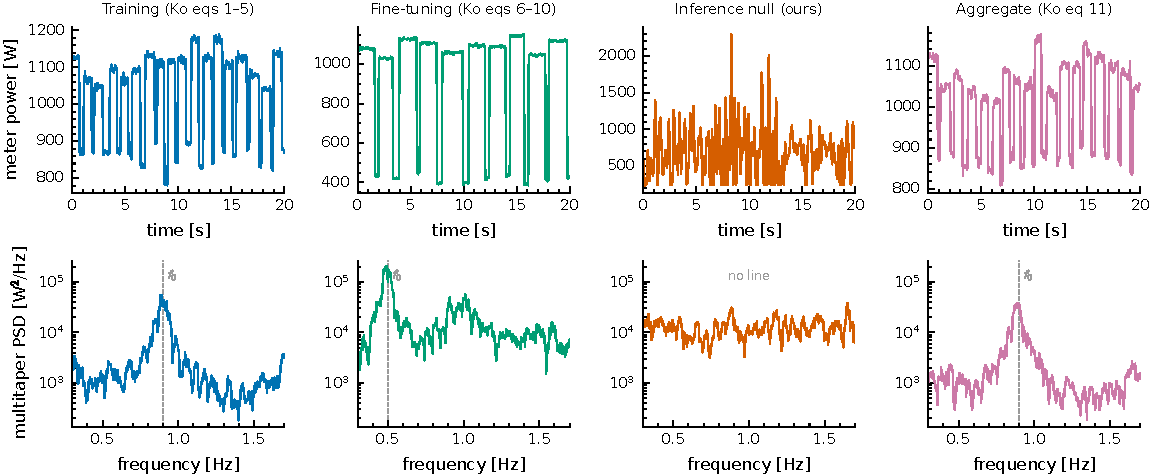
\includegraphics[width=\linewidth]{scenario_traces}
	\caption{The four workload classes at the meter, on the nominal channel
	(20\,Hz sampling, no filtering or decimation, $\sigma_\eta = 4$\,W). Top:
	a 20\,s excerpt. Bottom: the multitaper spectrum over the
	$0.3$--$1.7$\,Hz search band, with the true cadence marked. Training,
	fine-tuning, and the aggregate carry a line at $f_0$; the inference null
	does not. It is not quiet --- it puts roughly three times the training
	in-band power into the same band --- but that power is spread, so its
	peak-to-median contrast is $3.2$ against $44$ for training. A matched
	filter sees a raised floor and a tracker finds no path to follow. Cadences
	are pinned for legibility ($f_0 = 0.9$\,Hz training, $0.5$\,Hz
	fine-tuning); elsewhere they are drawn from the Ko bands.
	Reproduced by \texttt{scripts/plot\_scenario\_traces.py}.}
	\label{fig:scenario_traces}
\end{figure*}

\subsection{Adopted: the Ko--Zhu workload model}
\label{subsec:ko}

The training and fine-tuning waveforms are Ko and Zhu's
\citep{ko2025widearea}, taken with their published parameters. Training is a
two-phase iteration cycle: a compute up-phase at high operation rate followed
by a communication down-phase at low rate, with the period jittered
multiplicatively about a cadence $f_0$ drawn uniformly from $0.5$--$1.5$\,Hz,
the phase ratio drawn per iteration, and both levels perturbed. Fine-tuning is
the same engine on a second parameter set, with a lower cadence band and a
deeper tail-to-idle swing. The aggregate is their superposition: one dominant
training run at nine parts, against a background of smaller trainings and
fine-tunings at half a part each, all at one meter.

Two adaptations are worth stating. Ko and Zhu write the compute/communication
phase ratio as $r$; we reserve $r$ for the energy cost per operation of
\cref{eq:device} and write the ratio $\rho$. And their intra-phase fluctuation
term is a sub-millisecond effect: a meter integrating at tens of hertz averages
it far below one sample, so carrying it at full amplitude into a time-resolved
detector would be a modelling error rather than fidelity. We scale it down and
let the residual enter through the meter-noise channel of \cref{eq:meter},
which is where an off-chip instrument actually sees it.

We adopt this layer rather than inventing one for a specific reason. Ko and
Zhu's model was developed for grid-stability analysis and independently
reviewed by operators at AWS and Meta, so the training signature we detect is
not a signature we designed to be detectable.

\subsection{Constructed: the inference null}
\label{subsec:null}

Ko and Zhu model training, fine-tuning, and their aggregate. They do not
supply an inference workload, and Rung~2 needs one: without a stated
alternative, ``this trace is training-like'' has no content. We therefore
construct an inference null in the same power and superposition framework,
parameterised from the LLM-serving literature rather than from Ko and Zhu.

It superposes three structures. A decode floor, modelled as band-limited noise
over $0.1$--$4$\,Hz, stands for continuous batching
\citep{yu2022orca,kwon2023vllm}: the per-step cadence exists, but the batch
composition reshuffles every step, so the cadence smears into broadband in-band
power with no coherent frequency path. A slow Ornstein--Uhlenbeck envelope with
a $5$\,s correlation time and $40\%$ depth stands for expert-load imbalance
under sparse routing \citep{shazeer2017moe}; amplitude modulation spreads the
decode energy into sidebands, which makes the null \emph{harder}, not easier.
Prefill bursts arrive as a Poisson process at $0.08$\,Hz; memoryless arrivals
carry no line and simply raise the broadband in-band level.

The design intent is that none of the three carries a line. That is what makes
the null hard and what \cref{fig:scenario_traces} verifies: the null delivers
more in-band power than training while showing an order of magnitude less
spectral contrast. We also build an inference-dominant aggregate, substituting
this process into the dominant slot of Ko and Zhu's superposition at the same
power share. The two aggregate classes are then power-matched and both contain
the background's weak lines, so a detector must find the \emph{dominant} line,
not merely any line.

Everything downstream inherits the conditionality this creates. Rung-2
conclusions (\cref{sec:classification}) hold against this null, and a prover
running an inference workload with structure we have not modelled is outside
what those conclusions cover.

\subsection{Constructed: cadence wander and the adversary operators}
\label{subsec:generator_attacks}

Two further additions are ours. The first is honest: a slow
Ornstein--Uhlenbeck walk of the cadence itself, since a real training run's
iteration rate drifts with data, checkpointing, and contention. This is not an
attack, and it is the axis on which fixed-frequency detectors fail first.

The second implements the adversary operators of
\cref{subsec:adversary} inside the generator, so that each attack costs what
the physics says it costs rather than being applied as a post-hoc filter. Work
variation quantises the up-phase into an integer number of gradient-accumulation
micro-steps and varies that count, which moves real work; crucially the
down-phase keeps its honest draw, because a synchronous exchange does not
shrink because the preceding compute phase was shorter. Phase slip diffuses
iteration boundaries by a Brownian increment while holding the target period
fixed --- distinct from Ko and Zhu's jitter, which draws independent periods
and so ties boundary diffusion to the period variance. Harmonic smoothing
convolves the level waveform with a raised cosine, ramping transitions so the
harmonic comb dies while the fundamental survives. Shape filling raises the
down-phase level toward the up-phase, collapsing the swing at matched mean
power. \Cref{sec:frontier} prices each of these.

\subsection{Constructed: the observation map}
\label{subsec:obsmap}

The generator produces an operation rate $F(t)$; the device map of
\cref{eq:device} turns it into device power, and the observation map of
\cref{eq:meter} turns that into what a verifier reads. The implemented axes
are: a Butterworth low-pass standing for power-delivery and reporting
bandwidth; a trailing boxcar integration window; zero-order-hold decimation
onto a slower sample grid, deliberately without an anti-alias filter so that
aliasing is representable; an in-band notch of tunable depth and $Q$ for a
transfer-function anti-resonance near the cadence; a stable gain; additive
white or AR(1) meter noise; Ornstein--Uhlenbeck baseline wander; and a
square-wave controller limit cycle whose instantaneous frequency itself
wanders. One honest limitation: the realised quantisation is temporal --- the
integration window and the sample grid --- as there is no amplitude-quantisation
knob in the model.

The default configuration is an exact identity: with every axis off the map
returns the device trace unchanged and consumes no randomness. That is what
makes a one-axis-at-a-time sweep interpretable, because any movement is
attributable to the axis being swept.

\Cref{fig:scenario_meter} runs that sweep on a fixed honest training workload,
reporting how much of the cadence survives as the ratio of spectral power at
the known $f_0$ to the in-band power the meter itself contributes. All six axes
degrade it, and two extinguish it outright within the range a real instrument
might occupy: a $1$\,s integration window and a $1$\,Hz sample rate. This is a
statement about the signal in the channel, not about any detector. What each
detector class does with what survives --- and hence the minimum meter
specification --- is \cref{subsec:meter_spec}.

\begin{figure*}[t]
	\centering
	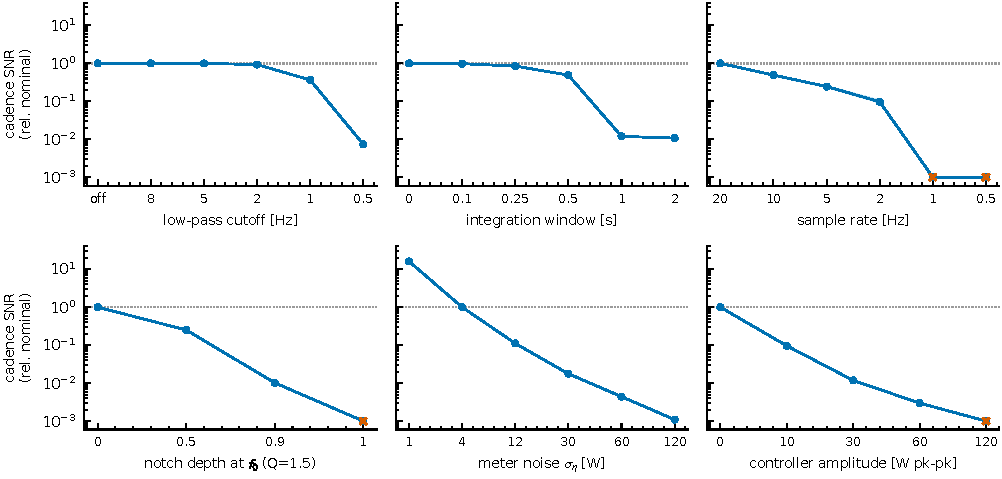
\includegraphics[width=\linewidth]{scenario_meter}
	\caption{Sensitivity of the cadence signature to the observation map, one
	axis at a time on a fixed honest training workload ($f_0 = 0.9$\,Hz, 20
	realisations, median and interquartile range). The measure is spectral
	power at the known $f_0$ over the in-band power the meter itself
	contributes, normalised to the nominal channel, so that attenuating axes
	act on the numerator and additive ones on the denominator and every panel
	reads the same way: down is worse for the verifier. Crosses mark settings
	where the cadence is not observable at all. Note $f_0$ is pinned away from
	$1.0$\,Hz, which would coincide with both the $2$\,Hz Nyquist frequency and
	the first sinc null of a $1$\,s boxcar. Reproduced by
	\texttt{scripts/plot\_scenario\_meter.py}.}
	\label{fig:scenario_meter}
\end{figure*}

\subsection{Sensitivity, not calibration}
\label{subsec:sensitivity}

The generator is literature-parameterized, not calibrated. The distinction is
load-bearing, and the evidence for it is our own: Ko and Zhu's model assumes an
iteration-cadence modulation of roughly $30\%$ of power, whereas we measure
about $0.40\%$ of board power at the corresponding frequency on a single A100
--- a gap of some $75\times$ (\cref{sec:reality}).

That gap is a scale and instrument limit rather than a modelling error. Ko and
Zhu's deep modulation is a datacentre-aggregate effect driven by distributed
synchronisation, which a single saturated card does not exhibit because it has
no communication phase; and the on-device telemetry we measured through is
itself a smoothed, roughly $10$\,Hz channel. The cadence is real at every
scale; its power signature is collective. Since the parameters were not fitted
to measured hardware, we do not claim they were, and we report sensitivity
analyses instead: results are stated as a function of the generator and
observation-map parameters rather than at a single privileged operating point.
(The word ``calibration'' appears elsewhere in this paper in an unrelated
sense --- the per-trace surrogate calibration of the detector null in
\cref{subsec:st1} --- which concerns a test's false-alarm rate, not the
generator's fidelity to hardware.)

\subsection{The transfer family}
\label{subsec:transfer}

Finally, we fix the population over which \cref{sec:classification} tests
domain shift. Six shifts move one factor each away from the nominal setting:
device headroom down to $0.70$ and up to $0.95$ of peak; observation duration
halved to $150$\,s, which halves the frequency resolution; the cadence band
shifted up to $0.8$--$1.8$\,Hz, so its top now lies outside the
$0.3$--$1.7$\,Hz search band; a meter carrying the controller limit cycle; and
a meter with heavy coloured noise and baseline wander. Decision rules are
fitted on the nominal population and evaluated on the shifted one zero-shot.

% ============================================================================
\section{Structural evidence (Rung 1)}
\label{sec:structural}
% ============================================================================

Rung 1 asks the weakest question on the ladder: does the trace carry
order-coherent power variation that a stated structural null does not produce?
Rejecting the null establishes \emph{coherent repeated power structure}, not
training: reading that structure as repeated multi-phase computation
additionally requires the nuisance model of \cref{sec:threat} that excludes
periodic physical confounds, of which the measured A100 power-controller
oscillation (\cref{sec:reality}) is the standing counterexample. Rung 1 is
evidence, not identification. We treat two prover settings in turn: a benign
prover whose cadence is stationary, and an adaptive prover who lets the cadence
wander to hide it. The benign case is easy, and the paper is not about the
benign case; the adaptive case is the methodological heart, and the burden of
this section is to show that its detector has a defensible null.

\subsection{Benign setting: the qualified baseline}
\label{subsec:benign}

When the cadence is stationary, a repeated iteration structure appears as a
line, or a harmonic comb, in the power spectrum, and the natural test is the
Thomson multitaper harmonic F-test \citep{thomson1982multitaper,
percival1993spectral}. At a fixed frequency $f$ the statistic $F(f)$ is
distributed as $F(2, 2K-2)$ under a locally smooth Gaussian spectral null with
$K$ tapers, so the test is \emph{approximately pivotal under a stationary,
locally smooth spectral null}. It is not an exact false-alarm guarantee across
arbitrary external power traces: coloured baselines, controller interference,
and co-resident load all violate the local-smoothness premise. Because the
prover's cadence is not known a priori, the test must search a band of
candidate frequencies and harmonics, which requires a search correction.

The analytic correction is itself unreliable. Sweeping the padded frequency
grid and applying a Bonferroni correction over the Rayleigh-resolution cell
count is \emph{anti-conservative by a factor of roughly $3.6$--$6\times$},
uniformly across our null suite: the maximum of $F$ over the padded grid
behaves like about five times more effective independent tests than the
Rayleigh count, because the $F$ ratio fluctuates below the Rayleigh scale. The
analytic multitaper tail is therefore usable only as a ranking statistic; its
operative false-alarm calibration is the Monte-Carlo one supplied by the
harness of \cref{subsec:st1}. A spectral matched filter (peak PSD at the
searched cadence) serves as the simple comparator. Both are honest baselines
for a stationary line, and both fail the moment the line wanders: as the
bake-off of \cref{app:bakeoff} shows, the fixed multitaper F-test retains
essentially no usable detection power once the cadence drifts, which is exactly
why the adaptive setting needs a different detector.

\subsection{Adaptive setting: tracked cyclostationary detection}
\label{subsec:tracked}

An adaptive prover breaks the benign baselines cheaply by letting the cycle
frequency wander, smearing the line across the searched band. We restore
coherence by estimating the wander and undoing it before testing. The detector
has three components, each with one job. First, a tracker estimates the
instantaneous cycle frequency $\hat f_0(t)$ from the time--frequency plane; the
tracker is a nuisance-parameter estimator, \emph{not} the detector. Second, the
phase estimate
\begin{equation}
	\hat\theta(t) \;=\; 2\pi \int_0^t \hat f_0(s)\,\mathrm{d}s
	\label{eq:phase}
\end{equation}
defines a resampling of the trace at equal increments of $\hat\theta$
(tacholess order tracking \citep{bonnardot2005tacholess}), so a wandering line
becomes a constant-order line. Third, the de-warped signal is tested for
cyclostationarity at candidate cycle frequency $\alpha$ with the
Dandawat\'e--Giannakis statistic \citep{dandawate1994cyclostationarity}
\begin{equation}
	Q_\alpha \;=\; N\, \hat r_\alpha^{\mathsf{H}}\, \hat\Sigma_\alpha^{-1}\, \hat r_\alpha,
	\label{eq:dg}
\end{equation}
where $\hat r_\alpha$ collects the estimated cyclic autocovariances at lags
$\tau$ and $\hat\Sigma_\alpha$ is a consistent estimate of their long-run
covariance. For a \emph{fixed} $\alpha$, $Q_\alpha$ is asymptotically
$\chi^2_{2L}$ under the structural null, given weak dependence, consistent
covariance estimation, and regularity.

Those conditions do not automatically cover the complete adaptive pipeline. The
tracker performs an effective search over frequency paths (a look-elsewhere
effect); the time warp is estimated from the same record it tests; the
covariance estimator $\hat\Sigma_\alpha$ must be chosen; and the asymptotic
$\chi^2$ tail may be a poor guide at finite length. Whether the null survives
these steps --- and in what form it can be claimed --- is the make-or-break
question of \cref{subsec:st1}. We do not call the adaptive pipeline an analytic
CFAR detector; \cref{subsec:st1} establishes what it is instead.

\subsection{Null validity of the complete pipeline}
\label{subsec:st1}

The question is whether the adaptive pipeline has a null we can defend. We
answer it with a staged design that isolates each adaptive ingredient in turn,
crossed with a graded suite of nulls, and measured by the realised false-alarm
rate at operationally small nominal levels --- not only $0.05$. The four stages
add one adaptive step at a time: (1) a fixed cyclic frequency $\alpha$ with no
resampling; (2) resampling under a \emph{known} independent time warp; (3) a
warp \emph{estimated} on held-out blocks and scored only on the complement; and
(4) the fully adaptive full-trace Viterbi tracker. The null suite grades from
stationary Gaussian and coloured processes (white, AR(1), a resonant AR(2)),
through stationary non-Gaussian processes (heavy-tailed, skewed, squared
Gaussian), to locally stationary and controller-like processes (a
Van~der~Pol--type power-management limit cycle mimicking the measured A100
controller). Each cell draws $M=10^4$ null traces; realised rates carry
Clopper--Pearson $95\%$ intervals. \Cref{fig:st1_far} shows the whole grid.

\begin{figure*}[t]
	\centering
	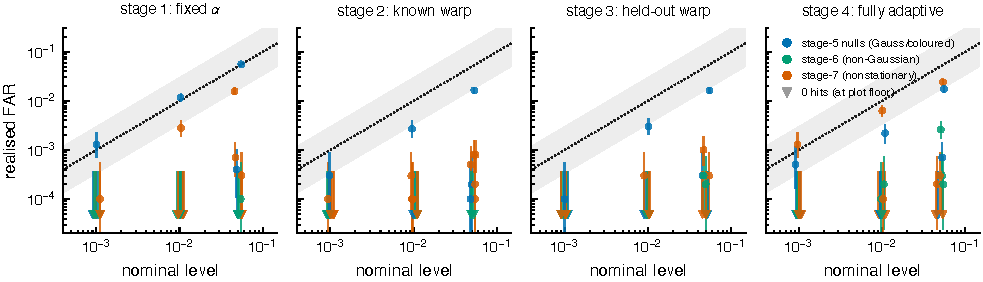
\includegraphics[width=\linewidth]{st1_calibration_far}
	\caption{Realised versus nominal false-alarm rate for the adaptive
	pipeline (Dandawat\'e--Giannakis with a Bartlett HAC covariance), one panel
	per stage, every null in the suite, with Clopper--Pearson $95\%$ intervals;
	nulls are coloured by stage group. No stationary null exceeds the nominal
	rate at any stage: the two-sided miss is \emph{deflation}, never
	inflation.}
	\label{fig:st1_far}
\end{figure*}

\paragraph{Level safety holds everywhere.} Across the entire campaign no
stationary Gaussian, coloured, or non-Gaussian null inflates the realised rate
at any stage or level: the failure mode the gate was built to catch ---
adaptivity silently raising the false-alarm rate --- does not occur. On the
white null the fixed-$\alpha$ stage is near nominal ($0.056$, $0.012$, and
$0.0013$ at nominal $0.05$, $10^{-2}$, and $10^{-3}$); on coloured and
non-Gaussian nulls the same stage is strongly conservative (realised rate
$\approx 0$). Tracing the three adaptive steps on the white null, where the
fixed-$\alpha$ stage was near nominal, isolates what each one does:
\begin{itemize}
	\item \textbf{Resampling alone (stage 1$\to$2)} deflates the rate by about
	$3.4\times$ ($0.056\to0.016$ at nominal $0.05$). Interpolating onto the
	angle grid correlates adjacent samples, the Bartlett estimator reads that
	as extra dependence and inflates $\hat\Sigma_\alpha$, and $Q_\alpha$
	shrinks. Resampling \emph{colours} the series.
	\item \textbf{Estimating the warp (stage 2$\to$3)} moves the null nowhere
	($0.016\to0.016$): the held-out design does what it promises.
	\item \textbf{Path selection (stage 3$\to$4)} adds no significant
	inflation ($0.016\to0.018$; every interval pair overlaps). Even on the
	resonant AR(2) null, which the Viterbi tracker provably locks onto, the
	fully adaptive stage fires never in $10^4$ traces: locking onto a broad
	noise resonance does not manufacture the phase-coherent cyclic structure
	$Q_\alpha$ requires.
\end{itemize}
The adaptive pipeline is therefore level-safe end to end. What fails is strict
two-sided coverage: after resampling the pipeline is uniformly conservative,
and the null $p$-values are not uniform (Kolmogorov--Smirnov uniformity is
rejected at every adaptive cell).

\paragraph{No analytic calibration closes the deflation.} We swept the open
choices --- record length, lag set, taper bandwidth, search band, interpolation
scheme, and the covariance estimator --- selecting on null-calibration quality
across the suite, never on power. Only the covariance estimator moves the
deflation, and it cannot be closed for the whole ladder at once
(\cref{fig:st1_cov}). Widening the Bartlett bandwidth to $b=54$ repairs the
adaptive stage two-sided (AR(1) realised $0.050/0.012/0.0016$ across the three
levels) --- confirming that the deflation is an under-bandwidth artefact of the
oscillating autocovariance of the resampled series --- but the \emph{same}
bandwidth breaks the fixed-$\alpha$ anchor, inflating white to $0.073$ at
nominal $0.05$. No single covariance configuration in the swept family
calibrates the ladder end to end, and Kolmogorov--Smirnov uniformity is
rejected at every adaptive sweep point regardless. The asymptotic $\chi^2$ tail
survives only as a level-safe, power-costing conservative bound; it is not a
calibration, and we do not report the adaptive pipeline as an analytic CFAR
detector.

\begin{figure*}[t]
	\centering
	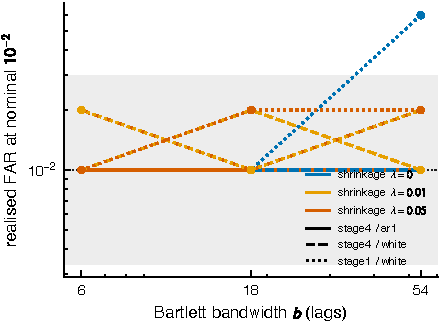
\includegraphics[width=\linewidth]{st1_calibration_cov}
	\caption{The covariance-estimator sweep is the fix-or-reframe axis:
	realised rate at nominal $10^{-2}$ versus Bartlett bandwidth $b$ for each
	shrinkage. The bandwidth that repairs the fully adaptive stage (stage 4)
	inflates the fixed-$\alpha$ anchor (stage 1). No single configuration
	calibrates both.}
	\label{fig:st1_cov}
\end{figure*}

\paragraph{Surrogate calibration recovers the null.} Running the entire
pipeline --- tracker, resampling, and test --- inside a Fourier-phase surrogate
null (which preserves the power spectrum and randomises phases, encoding the
linear-stationary invariance) recovers exact calibration where the asymptotic
tail was $3$--$6\times$ conservative. On the stationary Gaussian nulls the
realised rate covers nominal across all three pipeline stages --- fixed-$\alpha$,
held-out-warp, and fully adaptive (at nominal $0.05/10^{-2}$: white
$0.051/0.009$, AR(1) $0.050/0.013$ fixed-$\alpha$; white $0.052/0.013$, AR(1)
$0.054/0.010$ fully adaptive; the resonant-AR(2) and held-out-warp cells likewise)
--- and Kolmogorov--Smirnov uniformity is not rejected, the property the analytic
$p$-values never achieved.\footnote{Frozen on the MATS compute cluster over
stages 1/3/4 $\times$ eight nulls at the surrogate sizing $M=2000$ null traces
$\times$ $S=999$ surrogates (the level-safety and bake-off numbers above are at
$M=10^4$; surrogate cells are capped lower because each carries $S$ inner
resamples). This supersedes the earlier partial $M=1000$/$S=199$ grid. The
heavy-tailed but \emph{linear} non-Gaussian nulls stay level-safe (conservative:
$t$-innovation AR(1) $0.037/0.005$, log-normal $0.035/0.006$ fully adaptive); the
one exception is the \emph{nonlinear} squared-Gaussian null, which the fully
adaptive stage over-rejects mildly ($0.087/0.018$, ${\approx}1.7\times$, below the
pre-registered $3\times$ threshold). Its cause is the same linear-stationarity
assumption analysed next for the controller: a Fourier-phase surrogate cannot
reproduce the quadratic phase structure of a squared process and so under-spreads
the null. The level-safety claim is thus scoped to linear-stationary nulls.} This
is what ``calibrated'' means throughout the paper: an effective score with
per-trace surrogate calibration, not an analytic guarantee.

\paragraph{The controller marks the attribution boundary.} The surrogate null
encodes linear stationarity, so a genuine limit cycle --- which is itself
cyclostationary --- must and does inflate it: on the measured-controller null
the surrogate-calibrated rate rises to $0.17$--$0.30$ at nominal $0.05$. This is
not a defect. The detector correctly reports coherent cyclic structure in a
controller trace; calling that structure \emph{training} is the causal-attribution
step that needs the nuisance model of \cref{sec:threat}. The controller is the
periodic physical confound that Rung~1 alone cannot exclude, and its
false-alarm behaviour is exactly the ceiling the claim ladder assigns to this
rung. The separation that Rung~1 \emph{can} deliver --- power against this
confuser class, not merely against inference --- is quantified by the bake-off
of \cref{app:bakeoff}.


% ============================================================================
\section{The de-periodicisation frontier}
\label{sec:frontier}
% ============================================================================

Rungs 1 and 2 assume the prover leaves a recoverable cadence. An adaptive
prover need not: it can de-periodicise its schedule to smear that cadence away.
The question this section answers is not whether de-periodicisation is possible
--- it always is --- but how far a prover must go before the meter loses the
signal, and what that costs. This is a central result of the paper, not a
caveat, and its shape is not the naive one. De-periodicising is not
automatically cheap: some ways of doing it cost throughput without buying any
concealment, and the interesting question is whether \emph{any} way is both
cheap and effective.

We sweep six attack families as operators on the training schedule
(\cref{subsec:adversary}) --- per-iteration duration jitter, slowly drifting
cadence, variable real work per iteration, cadence relocation toward the
search-band edge, harmonic suppression, and dilution by co-resident load --- plus
a meter-degradation family treated separately in \cref{subsec:meter_spec}. For
each family we step an attack level and, at every level, measure the physical
de-periodicisation it induces (cadence coefficient of variation, phase
diffusion) against detector power for the tracking class (the Viterbi tracker
and the tracked Dandawat\'e--Giannakis order statistics) and for the fixed class
(the spectral matched filter and the multitaper F-test), all at nominal
false-alarm rate $0.05$ with $n=200$ traces per class. Where an attack has a
measured systems cost we attach it from the single-A100 throughput anchors
(\cref{sec:reality}); the plausible \emph{learning-efficiency} penalty
--- batch-size, accumulation, or update-timing changes that preserve tokens per
second while worsening progress per token or per joule --- is not something a
synthetic power model can measure, and we carry it as the standing open
empirical question rather than a result.\footnote{Frozen on the MATS compute
cluster (slurm array 5635), $n=200$ per class over $50$ cells, seed $0$, the full
five-detector set; \texttt{results/st2/frontier\_summary.json}
(\texttt{provisional=false}). The systems-cost axis reads only the clean
throughput-overhead field of the measured campaign, not its signature-B line-band
arrays, so the frontier is unaffected by the transport caveat of
\cref{sec:reality}.}

\paragraph{The costly attacks are the wrong ones.} The de-periodicisations that
degrade the line most are exactly the ones a rational prover would not pay for.
Idle-insertion jitter buys no concealment: it costs $15$--$375\%$ throughput and
leaves the tracked line detectable. Slowly drifting the cadence costs up to
${\sim}140\%$ and is precisely the regime the order tracker was built to survive
(\cref{app:bakeoff}). Power shaping costs $170$--$230\%$. Against every one of
these the tracking class holds while the prover pays a throughput tax that a
compute-governance regime would itself flag.

\paragraph{The cheap attack collapses the fixed tests but not the tracker.} The
dangerous family is variable real work. Varying the useful computation performed
per iteration moves the cadence without inserting idle time, so its throughput
cost is essentially zero: at work-variation level $0.35$ and $0.5$ the measured
overhead is $-0.10\%$ and $-0.36\%$ --- zero within noise. At that price the
fixed tests are gone. The spectral matched filter falls to detection rate $0.26$
and $0.27$ (its \textsc{auc} collapses to $0.44$ and $0.41$, below chance), and
the multitaper F-test sits at its floor. Yet the Viterbi tracker holds detection
rate $1.0$ at both levels (\cref{fig:frontier,fig:st2_work}). This is the genuine
scope boundary of the passive channel: a prover willing to vary real work evades
every cheap, fixed detector at no measurable systems cost, and only an
order-tracking detector still sees the schedule.

\begin{figure*}[t]
	\centering
	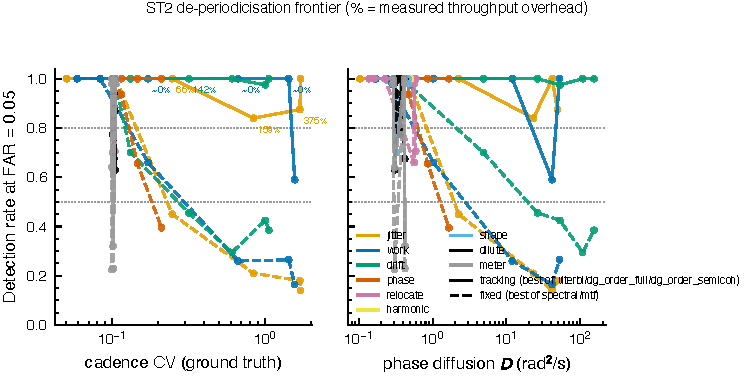
\includegraphics[width=\linewidth]{st2_frontier}
	\caption{The de-periodicisation frontier: physical de-periodicisation
	(cadence coefficient of variation) against best tracking and best fixed
	detector power at nominal false-alarm rate $0.05$, over all attack families.
	The near-vertical drop of the fixed class at the variable-real-work family,
	at essentially zero throughput cost, while the tracking class holds, is the
	scope boundary; costlier families (idle jitter, drift, shaping) sit at high
	throughput overhead without erasing the tracked line.}
	\label{fig:frontier}
\end{figure*}

\begin{figure*}[t]
	\centering
	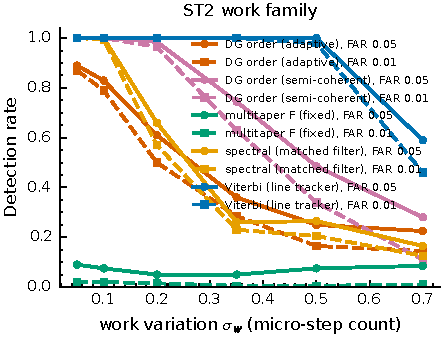
\includegraphics[width=\linewidth]{st2_work}
	\caption{Detector power versus variable-real-work level for each detector.
	The fixed matched filter and multitaper F-test cross below chance by level
	$0.35$; the tracked order statistics degrade more slowly; the Viterbi
	tracker holds full power until it finally bends at level $0.7$ (detection
	rate $0.59$) --- a level whose throughput and learning cost we do not
	measure.}
	\label{fig:st2_work}
\end{figure*}

\paragraph{The tracker's own boundary is unmeasured.} The Viterbi tracker does
eventually bend --- at work-variation level $0.7$ its detection rate falls to
$0.59$ --- but we do not report that as a defeat, because we cannot price it. The
throughput cost of driving work variation that hard is not in the measured
anchors, and the learning-efficiency cost is the open question above. The honest
statement is therefore asymmetric: within the regime whose cost we can measure
(overhead within noise) the tracker wins outright, and the far end of the
frontier, where the tracker finally fails, is a cost we could not quantify rather
than a cost shown to be small. That the tracker's advantage here is real and not
a tuning artefact is established independently in \cref{app:bakeoff}: against the
inference null the Viterbi tracker is essentially Neyman--Pearson optimal, so the
fixed tests' collapse under variable work is a genuine loss of information from
the schedule, not a deficiency of a particular detector.

\paragraph{The trade-off itself.} Plotting hiding directly against measured cost
(\cref{fig:st2_cost_pareto}) separates the two detector classes sharply. Against
the fixed class the Pareto staircase reaches hiding $0.74$ at essentially zero
overhead and climbs only to $0.79$ at $159\%$ and $0.82$ at $375\%$ however much
the prover spends: the cheapest attack is within $0.08$ of the best one. Against the tracking class the
staircase never leaves the floor, rising only to $0.16$ and doing so at $159\%$
overhead, so no attack in the anchored set buys meaningful concealment from the
tracker at any price we can measure. Reading the two panels together is the
paper's central empirical claim in one figure: what the fixed tests lose for free,
the tracker keeps at every measured cost. The figure also shows the boundary of
that claim honestly. Only $16$ of the $50$ swept cells have a measured hardware
cost anchor, and the rest --- including work-variation level $0.7$, where the
tracker finally bends --- carry no price at all, so they appear in a separate
unpriced strip rather than being dropped.

\begin{figure*}[t]
	\centering
	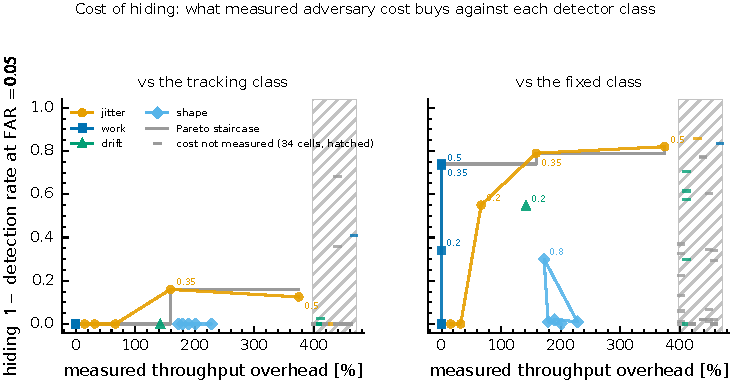
\includegraphics[width=\linewidth]{st2_cost_pareto}
	\caption{Cost of hiding: measured throughput overhead against hiding
	($1-$ detection rate at false-alarm rate $0.05$) for the four cost-anchored
	attack families, with the Pareto staircase --- the best hiding available at or
	below a given cost. Against the tracking class (left) the staircase stays on
	the floor across the whole measured cost axis; against the fixed class (right)
	the variable-real-work family reaches hiding ${\sim}0.74$ at zero cost. Cells
	whose attack level has no hardware cost anchor cannot be placed on the cost
	axis and are shown in the hatched strip, among them the level at which the
	tracker itself begins to fail. Attack levels are labelled where they hide
	something; the rest sit on the floor.}
	\label{fig:st2_cost_pareto}
\end{figure*}

\paragraph{Governance reading.} A passive meter certifies efficient
iteration-structured training against cheap, fixed tests only within a bounded
de-periodicisation budget; a prover free to vary real work escapes those tests
for nothing. Defeating the order tracker on top of that requires either a systems
and learning cost we could not measure or a degradation of the meter channel
itself (\cref{subsec:meter_spec}). The results of this section are therefore
necessary conditions and an upper bound on hideability rather than a proof of
training: they bound what a prover can hide from a fixed detector cheaply. The
complementary direction --- a lower bound on what hiding must cost, which no
detection sweep can supply --- is available for one attack family against a fixed
verifier (\cref{prop:sigmastar}) under the cost assumption of \cref{ass:cost},
and the distortion it requires can be priced against the same anchors used here.
The tracking class dominates the fixed class at every cell we measured, so that
threshold is a valid --- but loose --- reading of what a tracker would require: it is
read off the weaker detector, so it understates the true requirement. Establishing it
against the tracking class directly, rather than inheriting it from the measured
dominance, remains open.

\subsection{A minimum meter specification}
\label{subsec:meter_spec}

The frontier above assumes a meter that resolves the cadence band. The
verifier's instrument is itself an attack surface: a prover who cannot
de-periodicise cheaply may instead argue for, or be handed, a meter too coarse
to see the line. We therefore sweep the meter rather than the schedule --- sample
rate and integration window between the nominal $20$~Hz channel and a $1$~Hz
integrating sampler, plus transfer-function notch depth and position near the
cadence --- with honest training against the hard inference null, and locate where
each detector class dies.\footnote{Frozen on the MATS compute cluster (slurm
array 5498), $48$ cells, $n=200$, $300$~s traces;
\texttt{results/st2/meter\_boundary\_summary.json}. Marginal and dead-cell
\textsc{auc}s are sensitive to the BLAS build, but the live-region boundary is
not.} The result is a minimum specification the channel must meet for the Rung-1
and Rung-2 claims to hold, which we state as a channel requirement, not an attack
cost.

\paragraph{The specification.} The tracking class holds full power (detection
rate ${\gtrsim}0.9$ at nominal $0.05$) if and only if the meter satisfies three
conditions together (\cref{fig:meter_boundary}). First, a sample rate of at least
about $2$~Hz: rates of $20$, $10$, $5$, and $2$~Hz all hold the Viterbi tracker
near $1.0$, $1$~Hz collapses it to $0.36$ as the Nyquist edge crosses the band,
and $0.5$~Hz is dead (every detector at chance). Second, an integration window no
longer than about $0.5$~s: at $20$~Hz sampling a window of $0.5$~s still holds
($0.99$), but a $1$~s boxcar sinc-nulls the $1$~Hz band centre and collapses the
tracker to $0.25$ even at full sample rate. Third, no deep transfer-function
notch at the cadence: an off-band or shallow notch is tolerable (tracker
${\approx}1.0$), but a full-depth notch at $1.0$--$1.2$~Hz roughly halves tracker
power (to $0.48$--$0.55$) without erasing it (\cref{fig:meter_boundary_notch}).
The robustness ordering across the grid is Viterbi $\ge$ spectral $>$ the DG order
family, which is the most sensitive detector at the reference channel but the
first to die as the channel degrades; the multitaper F-test is at its floor
throughout.

\begin{figure*}[t]
	\centering
	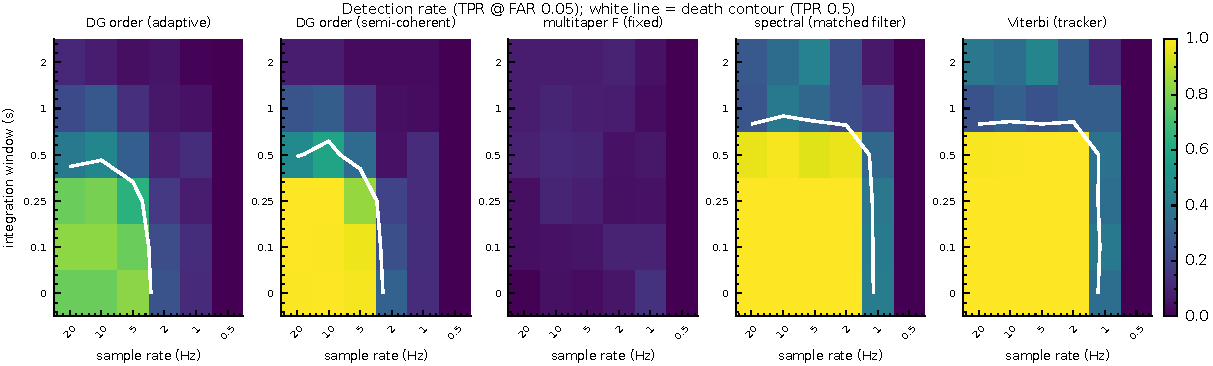
\includegraphics[width=\linewidth]{st2_meter_boundary}
	\caption{Minimum meter specification: detector power at nominal false-alarm
	rate $0.05$ over sample rate $\times$ integration window, one panel per
	detector, honest training against the hard inference null. The live region
	is sample rate ${\ge}2$~Hz \emph{and} integration window ${\le}0.5$~s; below
	either edge the tracking class collapses toward chance.}
	\label{fig:meter_boundary}
\end{figure*}

\begin{figure*}[t]
	\centering
	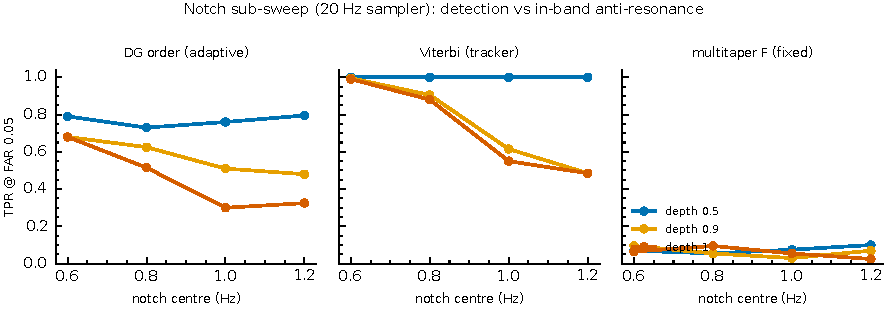
\includegraphics[width=\linewidth]{st2_meter_boundary_notch}
	\caption{Transfer-function notch sub-sweep at $20$~Hz sampling: tracker power
	versus notch centre frequency and depth. Only a deep notch placed at the
	cadence centre ($1.0$--$1.2$~Hz) materially degrades detection, and it halves
	rather than erases it.}
	\label{fig:meter_boundary_notch}
\end{figure*}

\paragraph{The frontier's meter-erasure point, decomposed.} This sweep also
resolves the single integrating-$1$~Hz point reported on the frontier, where even
the tracker degrades (Viterbi detection rate $0.32$, every other detector near
chance). That point superposes two independent channel defects, and the boundary
map shows either one suffices: at the reference channel the tracker is at $1.0$;
adding the $1$~s integration alone drops it to $0.25$; the $1$~Hz sampling alone
drops it to $0.36$; the two together give $0.30$. The meter-erasure regime is
over-determined --- it is a statement about the instrument, and a demand on it,
rather than a de-periodicisation attack the prover can mount for free.


% ============================================================================
\section{Conditional training classification (Rung 2)}
\label{sec:classification}
% ============================================================================

Rung 1 asks whether coherent iteration structure is present. Rung 2 sharpens
this into a decision: is a trace more training-like than a stated inference
population? A decision needs a reference, and ours is the modelled
continuous-batching inference null (\cref{sec:scenario}); every Rung-2 conclusion
is conditional on that null. We fix the task in advance --- the feature vector,
the decision rules, and the reporting --- so that the classification result is not
retrofitted to the answer.

\paragraph{Features and decision rules, specified in advance.} Each trace is
reduced to an eight-dimensional physics feature vector estimated \emph{from the
trace alone}, with no oracle knowledge of the cadence: the six Rung-1 detector
scores (multitaper F, harmonic comb, spectral matched filter, Viterbi, fixed-$\alpha$
DG, and tracked-order DG), plus two stability features read off the estimated
Viterbi path --- its frequency-path stability and its phase-folded waveform
repeatability. On this fixed vector we compare three decision rules of increasing
freedom: (i) a prespecified physics score, a fixed linear combination with the
fixed-cadence comparators pre-registered out; (ii) a logistic discriminant fitted
to the scenario generator and scored out-of-fold; and (iii) a random-forest
learned reference, included to expose how much separation comes from the chosen
null rather than from the structural method. We report area under the ROC curve
and the false-negative rate at a false-positive rate of $0.05$, kept separate
from the Rung-1 structural false alarms of \cref{subsec:st1}.\footnote{Frozen on
the MATS compute cluster (slurm array 5612), $n=200$ per class, $300$~s traces,
band $0.3$--$1.7$~Hz, $14$ cells (the stated population, six transfer shifts, and
seven semantic controls); \texttt{results/rung2/rung2\_summary.json}.}

\paragraph{Stated population and transfer.} On the stated population all three
rules separate training from the hard inference null perfectly: area under the
curve $1.00$ with zero false negatives at a false-positive rate of $0.05$
(\cref{fig:rung2_stated}). The separation is not brittle to the population. Across
six domain shifts --- a low and a high cadence peak, a shortened $150$~s record, a
cadence band shifted to $0.8$--$1.8$~Hz, a hostile controller-limit-cycle meter,
and heavy coloured meter noise --- the area under the curve stays $1.00$. The
physical schedule of efficient training is far enough from the inference null that
leaving the stated parameter box does not close the gap.

\begin{figure*}[t]
	\centering
	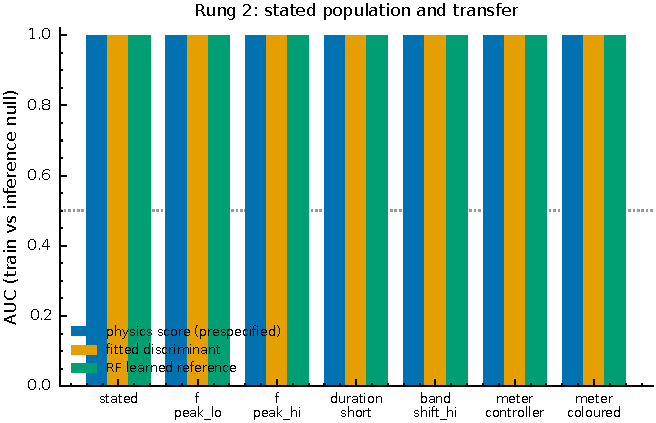
\includegraphics[width=\linewidth]{rung2_stated_transfer}
	\caption{Rung-2 classification on the stated population (ROC / operating
	points for the three decision rules) and across the transfer shifts. All
	three rules reach area under the curve $1.00$ on the stated population and
	hold it under every domain shift.}
	\label{fig:rung2_stated}
\end{figure*}

\paragraph{The semantic controls set the ceiling.} The controls are the point of
the rung. We built seven loads whose training status we know and asked what each
rule scores (\cref{tab:rung2_controls}). Five non-training loads --- a
discarded-update decoy that runs the full forward/backward/optimizer step and
throws the update away, a gradient-only computation, a training-shaped non-ML
kernel loop, a controller limit cycle, and a periodic inference request generator
--- \emph{all} score as training, at fraction $1.00$ under every rule. A genuine
training run diluted by an unrelated co-resident load is still caught ($1.00$).
The reading is the one the claim ladder assigns to this rung: from power alone the
verifier can certify a \emph{training-shaped periodic compute schedule}, not that
the computation is gradient-descent training rather than a mimic. This is the
semantic decoy, and it is the ceiling that motivates the active protocol of
\cref{sec:active}. The controller cycle scoring as training is the same
attribution boundary Rung~1 met in \cref{subsec:st1}: the structural signal is
real, and calling it training needs the nuisance model of \cref{sec:threat}.

\begin{table*}[t]
	\centering
	\small
	\caption{Semantic-control outcomes: fraction of each load scored as training
	at a false-positive rate of $0.05$, per decision rule. Five non-training
	loads all score as training; the only control the tracked rules degrade on is
	asynchronous (de-periodicised) genuine training, which they nonetheless
	mostly catch.}
	\label{tab:rung2_controls}
	\begin{tabular}{@{}lcccc@{}}
		\toprule
		Control load & Training? & Physics & Fitted & Learned \\
		\midrule
		Discarded-update decoy & no & 1.00 & 1.00 & 1.00 \\
		Gradient-only & no & 1.00 & 1.00 & 1.00 \\
		Non-ML kernel loop & no & 1.00 & 1.00 & 1.00 \\
		Controller cycle & no & 1.00 & 1.00 & 1.00 \\
		Periodic inference & no & 1.00 & 1.00 & 1.00 \\
		Co-resident mixture & yes & 1.00 & 1.00 & 1.00 \\
		Asynchronous training & yes & 0.72 & 0.55 & 1.00 \\
		\bottomrule
	\end{tabular}
\end{table*}

\paragraph{Asynchronous training: a robustness result, not a miss.} One control,
strongly de-periodicised genuine training, was pre-registered as an expected miss
--- the case scoped out of Rung 2. At $n=200$ it is not missed. The tracked
physics rule catches it (area under the curve $0.89$, $72\%$ flagged) and the
learned reference catches all of it ($100\%$); only the fitted linear discriminant
is weak ($0.75$, $55\%$). This is consistent with the tracker-robustness story of
Rungs 1 and 2: the asynchronous control de-periodicises by drifting the cadence
centre and slipping the phase, which leaves a wandering but still coherent line
--- exactly the regime order tracking was built to survive. We therefore report it
as a robustness result rather than the boundary. The genuine evasion is not slow
wander but the ${\approx}$zero-cost variable-real-work attack of
\cref{sec:frontier}, which moves the cadence \emph{without} leaving a coherent
line, and which is where the tracker actually bends.

\begin{figure*}[t]
	\centering
	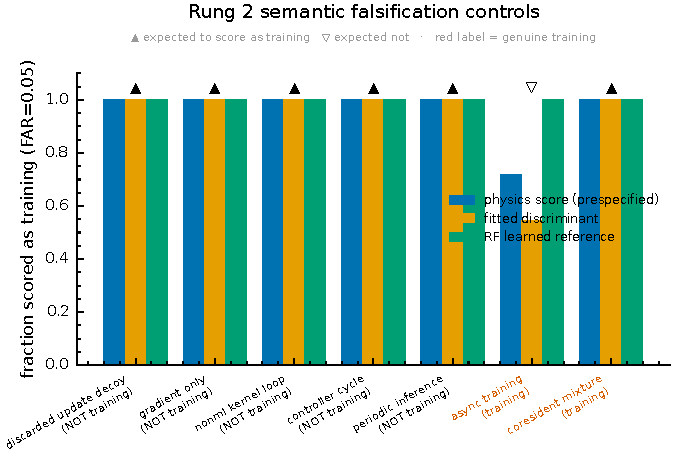
\includegraphics[width=\linewidth]{rung2_controls}
	\caption{Semantic controls: fraction scored as training per decision rule.
	The non-training decoys are indistinguishable from training under every rule
	(the semantic-decoy ceiling); only asynchronous genuine training separates
	the rules, and the tracked physics rule still catches most of it.}
	\label{fig:rung2_controls}
\end{figure*}


% ============================================================================
\section{From passive evidence to active authentication (Rungs 3--4)}
\label{sec:active}
% ============================================================================

% Plan §3.4. Default scope: concise conditional-protocol section (moves to an
% appendix if it distracts from Rungs 1–2); full empirical treatment only if
% the optional ST3 pilot runs and passes.

Rung 2 certifies the physical schedule, not training semantics. Its ceiling is
the semantic decoy: a load that reproduces the compute--communication cadence of
training without retaining a trained model scores as training under every passive
rule (\cref{sec:classification}). No passive test can separate the two, because
the meter sees only the schedule and the decoy copies the schedule. The way past
a passive ceiling is to stop watching and start asking. If the verifier perturbs
the machine and the machine must react, a decoy that merely replays a recording
cannot follow: it does not know what it was asked.

Rung 3 makes this concrete with a challenge-synchronous protocol. The verifier
emits an unpredictable balanced challenge sequence $c_k \in \{-1,+1\}$; the prover
runs a committed, semantically-equivalent variation of its training schedule keyed
to $c_k$ --- for instance a small pre-agreed shift in the boundary between two
iterations that leaves the computation performed unchanged. The verifier
correlates the external power trace against $c_k$ over a causal lag window, in the
manner of a lock-in amplifier or a spread-spectrum receiver recovering a known
code from noise. The null needs no corpus and no matched hardware: it comes from
re-randomising the challenge and recomputing the statistic. A positive result
authenticates a physical fact --- a load behind the meter responded to a signal it
could not have predicted. This escapes the semantic decoy, whose passive schedule
is by construction uncorrelated with the fresh challenge (\cref{subsec:adversary}).
Its own ceiling is the challenge-aware dummy load: a device that receives the
challenge and mimics the prescribed response without training.

The correlation test is exact under the sharp null that the challenge has no
effect on the measured process --- but only conditional on the randomisation
design, and the guarantee is fragile to the usual abuses
\citep{fisher1935design}. Any maximisation the verifier performs, over causal
lags, candidate impulse responses, or preprocessing choices, must be repeated
inside every re-randomised replicate, or the reported level is optimistic.
Carryover between challenge periods, any adaptivity in the prover's schedule
choices, and balance constraints on the challenge sequence all belong in the
design that the re-randomisation samples from. We also flag the weaker reading a
careless protocol invites: over a long enough record a correlation detector
accrues the $\sqrt{N}$ processing gain of any matched receiver, so a positive
result must be shown to certify the challenge binding and not merely that the
verifier integrated for long enough.

Rung 3 authenticates a physical response; it does not tie that response to
training. Rung 4 adds that binding, and it is the rung this paper does not build.
Rather than gesture at ``a proof of training,'' we state the missing piece as an
ideal functionality \citep{canetti2001uc}: a sound, fresh, challenge-bound
transcript or proof that ties each challenge bit to the prescribed
semantically-equivalent variation of declared training state transitions. Such a
primitive must provide commitment before the challenge is revealed,
unpredictability at commitment time, sound binding of the response to valid
declared state transitions, freshness against replay, and an explicit position on
whether the responding load and the declared computation are co-located.
Proof-of-learning constructions \citep{jia2021proofoflearning} are the closest
existing candidate, but they assume access to the training trace rather than an
external meter. Conditional on such a primitive, challenge-synchronous power
supplies physical evidence for the declared response; without it, the semantic
work binding remains an assumed, open layer.

Two ceilings therefore remain. Rung 3's is the challenge-aware dummy load;
Rung 4's is co-location: a genuine remote proof combined with a local
challenge-correlated dummy still satisfies both the correlation test and the
transcript unless the assumed primitive explicitly rules the separation out.
Closing them empirically is future work, and it needs no cluster --- challenge
modulation is legible on a single card. A full Rung-3 study would fix a concrete
pair of semantically-equivalent schedules, run the complete search inside every
re-randomised replicate, pit the detector against a challenge-aware dummy-load
adversary, and trace detection against modulation depth, throughput overhead, and
observation time. We leave it as the active-verification direction the passive
results here motivate but cannot reach --- the response to the ceiling that
\cref{prop:noident} makes unavoidable for any passive detector
(\cref{sec:discussion}).


% ============================================================================
\section{Reality check and transfer limits}
\label{sec:reality}
% ============================================================================

Every result above is synthetic. The one place we hold the scenario model
against measured hardware, it fails in an instructive way, and we report that
failure as a result rather than a closing nod.

\paragraph{The negative transport case.} On measured single-A100 traces the
iteration cadence is present but shallow: a saturated card has no communication
phase, so the iteration structure modulates a ${\sim}370$\,W draw by only a few
watts (${\sim}0.4\%$ of board power). Worse for the naive reading, the spectra
contain a $0.31$--$0.45$\,Hz component, roughly ten times stronger than the
training line, that appears whenever the load varies in time but not at idle or
under constant load --- the signature of the card's own power-management loop. It
is a hardware line that says ``time-varying load,'' not ``training,'' and it is
the standing counterexample that Rung~1 (\cref{sec:structural}) and the Rung-2
controller control (\cref{sec:classification}) are built to exclude.

\paragraph{Why this is the honest outcome.} Two things make the single-card
signature shallow. One saturated card has no synchronous communication barrier,
so the deep compute--communication contrast the scenario model assumes is absent;
and the generator is literature-parameterised, not calibrated to the measured
channel, a gap of about $75\times$ in modulation depth. The synthetic results are
therefore a sensitivity analysis over a plausible parameter family, not a
prediction calibrated to this hardware --- which is why the paper's claims are
scoped to the stated generator and its stated nulls throughout.

\paragraph{Falsifiable predictions.} The model makes two predictions we cannot
test here but state as falsifiable. Distributed synchronisation should deepen the
line: at cluster scale the periodic all-reduce barrier produces a deep, coherent,
legible cadence rather than the shallow single-card ripple, which is precisely the
physics \cref{ass:cost} leans on. And an
external wall or rack meter should see a different, lower-passed trace than
on-board NVML telemetry, shifting where the minimum meter specification of
\cref{subsec:meter_spec} binds. Both are predictions, not results.


% ============================================================================
\section{Discussion and conclusion}
\label{sec:discussion}
% ============================================================================

We set out to ask what a passive power meter can certify about AI training, and
organised the answer as a claim ladder in which each rung answers a more
governance-relevant question at a higher cost in verifier information, and each
rung's ceiling motivates the next. \Cref{tab:closeout} closes the ladder out with
the paper's evidence attached to each rung.

\begin{table*}[t]
	\centering
	\small
	\caption{The claim ladder closed out: what this paper establishes at each
	rung, where, and the hard ceiling it hits. Mirrors \cref{tab:ladder}.}
	\label{tab:closeout}
	\begin{tabular}{@{}p{2.4cm}p{5.0cm}p{2.2cm}p{4.6cm}@{}}
		\toprule
		Rung & What the paper establishes & Evidence & Demonstrated ceiling \\
		\midrule
		1. Structural evidence & Order-tracked cyclic structure is detected
		against stationary and controller-like nulls; the tracker is
		Neyman--Pearson optimal against the inference null &
		\cref{sec:structural}, \cref{app:bakeoff} & Fast cadence wander
		(${>}0.8$~Hz on $300$~s); attributing structure to training needs the
		nuisance model; the meter must meet \cref{subsec:meter_spec} \\
		2. Conditional classification & The trace is more training-like than the
		stated inference null (area under the curve $1.00$, stable across domain
		shift) & \cref{sec:classification} & The semantic decoy: non-training
		loads with a training-shaped schedule score as training; for the
		discarded-update decoy \cref{prop:noident} shows no passive detector can
		do better \\
		Frontier & Fixed tests collapse under ${\approx}$zero-cost variable real
		work while the tracker holds; costly de-periodicisations buy no
		concealment & \cref{sec:frontier} & The tracker's far end, at a systems
		and learning cost we could not measure \\
		Cost of hiding & Hiding to detectability $\varepsilon$ requires a
		distortion $\sigma^*(\varepsilon)$ that the measured anchors price at tens
		of percent of throughput, rising above $100\%$ (i.i.d.\ period jitter) &
		\cref{subsec:identifiability}, \cref{app:identifiability} & Read off a
		fixed-bin verifier, so valid against any class containing it, but loose;
		one attack family;
		internal to the stated generator; the throughput-or-learning disjunction is
		\cref{ass:cost}, not a result \\
		3--4. Active authentication & A challenge-synchronous protocol and an
		assumed binding primitive, specified but not run & \cref{sec:active} &
		Challenge-aware dummy load; the co-location gap \\
		\bottomrule
	\end{tabular}
\end{table*}

\paragraph{Scope.} The results are fixed-horizon: we make no claim that the
$\chi^2$ statistic supports anytime-valid monitoring, and defer sequential
e-process treatment. We use only the temporal-structure channel, excluding the
amount-of-computation and energy channels. The cryptographic binding of Rung~4 is
assumed as an ideal functionality, not built. Real distributed hardware enters
only as the falsifiable predictions and the negative transport case of
\cref{sec:reality}.

\paragraph{Limitations.} The scenario model is literature-parameterised, not
calibrated to measured hardware, so every quantitative result is a sensitivity
analysis over a stated parameter family; the ${\sim}75\times$ modulation gap of
\cref{sec:reality} is the standing reminder. The observation map is a
linear time-invariant first approximation. The optimality ceiling of
\cref{app:bakeoff} is optimal only under the Whittle model, hence a lower bound on
the true optimum. Every robustness claim is bounded by the attack families and
budgets we specified; a family we did not model is outside it. The cost bound of
\cref{subsec:identifiability} shares that limit: it covers i.i.d.\ period jitter,
and while it holds against any verifier class containing the test it exhibits, it is
obtained from a fixed-bin test and so reads loose against the order tracker our own
experiments show to be stronger --- it does not yet close the frontier's far end. Its cost leg is an
assumption (\cref{ass:cost}), not a result, for the reasons in
\cref{rem:costgap}. And the learning-efficiency leg of that bound --- the axis that would
turn it into a single priced statement rather than a disjunction --- is argued,
not measured, and remains the central open empirical question.

\paragraph{Governance reading.} What a regulator can buy today is graded. Rung~1
buys physical evidence of an efficient iteration-structured compute schedule from
an external meter alone, robust to a wander-and-drift adversary but not to a
prover who varies real work or degrades the meter. Rung~2 buys the further claim
that the schedule is more training-like than a stated inference baseline --- but
not that the computation is training rather than a schedule-matched decoy, which
is a limit of the passive channel, not of the method. Separating training from a
decoy, and binding a physical response to declared work, both require moving off
the passive channel to the active protocol of \cref{sec:active} and the
cryptographic primitive it assumes. The passive meter is thus a cheap, deployable
front line that narrows the question and prices the cheap evasions, not a
stand-alone proof of training.


% ============================================================================
\bibliography{references}
\bibliographystyle{icml2026}

\newpage
\appendix
% Make cleveref render appendix section labels as "Appendix A" rather than
% "Section A"; the appendix body runs single-column.
\crefalias{section}{appendix}
\crefname{appendix}{Appendix}{Appendices}
\Crefname{appendix}{Appendix}{Appendices}
\onecolumn

\section{Detector bake-off}
\label{app:bakeoff}

The choice of detector for Rung~1 is an \emph{outcome} of a pre-registered
comparison, not an assumption. Before scoring any signal we fixed the detector
set, the conditions, and the metric, so that ``we present one method'' is a
finding rather than a choice. The detector set spans the natural alternatives:
the fixed multitaper harmonic F-test (\texttt{mtf}); a spectral matched filter;
the raw Viterbi tracker score; the fixed-$\alpha$ Dandawat\'e--Giannakis
statistic given the \emph{true} $f_0$ as an oracle; and three variants of the
tracked order pipeline --- split (held-out warp), full (fully adaptive pooled),
and semi-coherent (a per-block Fisher combination). We score positives (Ko
training traces) over a cadence-drift axis $f_0^{\mathrm{drift}} \in
\{0, 0.1, 0.2, 0.4, 0.8, 1.5\}$~Hz against two negative classes, each with its
own empirical false-alarm threshold: the modelled inference null, and a mixed
structural population (equal parts AR(1), heavy-tailed AR(1), and the measured
controller). With $n=200$ traces per class the $10^{-2}$ threshold rests on the
second-highest negative score --- a granularity we state rather than hide.
\Cref{fig:st1_bakeoff} plots the power curves; \cref{tab:bakeoff} gives the
detection rates at nominal false-alarm rate $10^{-2}$.

\begin{figure*}[t]
	\centering
	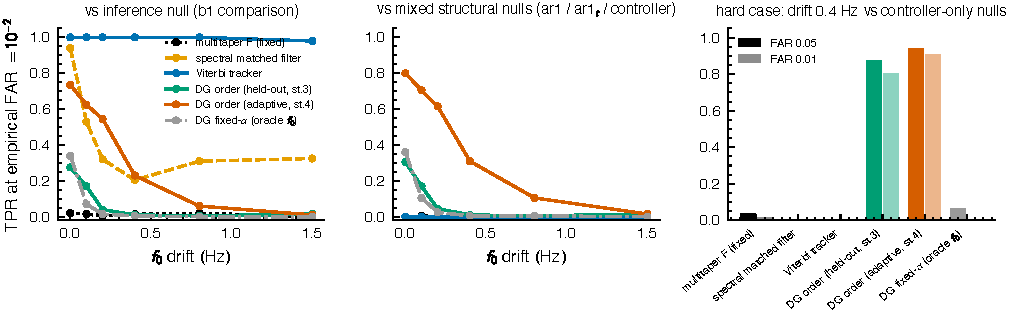
\includegraphics[width=\linewidth]{st1_bakeoff}
	\caption{Detector bake-off on the cadence-drift axis: detection rate at
	empirical false-alarm rate versus drift, for each detector and both
	negative classes. Only the tracked order family retains power against the
	structural negatives; the spectral-shape detectors detect the controller
	third of the mix more strongly than the signal.}
	\label{fig:st1_bakeoff}
\end{figure*}

\begin{table*}[t]
	\centering
	\small
	\caption{Bake-off detection rate at nominal false-alarm rate $10^{-2}$,
	by detector and cadence drift (Hz), against the inference null and the
	mixed structural population ($n=200$ per class).}
	\label{tab:bakeoff}
	\begin{tabular}{@{}lcccccc@{}}
		\toprule
		Detector & $0$ & $0.1$ & $0.2$ & $0.4$ & $0.8$ & $1.5$ \\
		\midrule
		\multicolumn{7}{@{}l}{\emph{vs.\ inference null}}\\
		\texttt{mtf} (fixed multitaper F) & 0.02 & 0.01 & 0.01 & 0.01 & 0.02 & 0.00 \\
		spectral matched filter & 0.94 & 0.53 & 0.32 & 0.20 & 0.31 & 0.33 \\
		Viterbi tracker & 1.00 & 1.00 & 1.00 & 1.00 & 1.00 & 0.98 \\
		DG order (split) & 0.28 & 0.17 & 0.04 & 0.01 & 0.01 & 0.01 \\
		DG order (full) & 0.73 & 0.62 & 0.55 & 0.23 & 0.06 & 0.01 \\
		DG order (semi-coherent) & 1.00 & 1.00 & 0.97 & 0.56 & 0.07 & 0.01 \\
		DG fixed-$\alpha$ (oracle $f_0$) & 0.34 & 0.07 & 0.01 & 0.01 & 0.00 & 0.00 \\
		\midrule
		\multicolumn{7}{@{}l}{\emph{vs.\ mixed structural nulls}}\\
		\texttt{mtf} & 0.00 & 0.01 & 0.00 & 0.00 & 0.01 & 0.00 \\
		spectral matched filter & 0.00 & 0.00 & 0.00 & 0.00 & 0.00 & 0.00 \\
		Viterbi tracker & 0.00 & 0.00 & 0.00 & 0.00 & 0.00 & 0.00 \\
		DG order (split) & 0.30 & 0.17 & 0.04 & 0.01 & 0.01 & 0.01 \\
		DG order (full) & 0.80 & 0.70 & 0.61 & 0.31 & 0.10 & 0.01 \\
		DG order (semi-coherent) & 1.00 & 1.00 & 0.99 & 0.69 & 0.14 & 0.03 \\
		DG fixed-$\alpha$ (oracle $f_0$) & 0.36 & 0.10 & 0.03 & 0.01 & 0.01 & 0.00 \\
		\bottomrule
	\end{tabular}
\end{table*}

Three findings follow, and they are the reason the main text presents a single
detector. First, \emph{tracking is necessary}: the oracle fixed-$\alpha$
statistic, handed the true $f_0$, collapses from $0.34$ at zero drift to
$\le 0.1$ under any wander --- even the true frequency is useless to a coherent
fixed-$\alpha$ test once the line moves --- and the fixed multitaper F-test has
essentially no usable power against either negative class at empirical
thresholds. Second, \emph{only the tracked order family separates the wandering
line from structural confounds}. Against the mixed structural negatives the
matched filter and the raw Viterbi score have detection rate zero at every
drift: the controller third of the mixture fires them harder than the signal
does, because a Viterbi score happily locks onto a limit cycle. The hard case
makes this sharp --- at drift $0.4$~Hz against controller-only negatives the
order pipeline holds $0.8$--$1.0$ detection at $10^{-2}$ while every
spectral-shape detector, including the fixed-$\alpha$ oracle, drops to near
zero. Phase-coherent cyclic structure at the tracked order is the one signature
the confuser cannot fake; this is the attribution boundary of Rung~1 drawn with
power, not false-alarm rate. Third, the \emph{semi-coherent variant dominates}
the pooled statistic at every drift, filling the fast-wander power hole up to
about $0.4$~Hz while remaining level-safe.

The honest boundary is fast wander. Beyond drift $0.8$~Hz every calibratable
detector fades (the semi-coherent variant falls to $0.07$--$0.14$ at
$10^{-2}$); only the raw Viterbi score keeps power against the inference null
there, and it cannot tell a training run from a controller. A $300$~s record
does not resolve fast cadence wander with an honest null. This is a scope
statement for the paper, not a repairable defect.

\paragraph{How far below optimal?} The bake-off ranks detectors against each
other; it does not say how good the winner is in absolute terms. Because we own
the generators, we can benchmark against an optimality ceiling: an approximation
to the Neyman--Pearson optimal test between the training and null generators. No
closed-form likelihood exists --- both are black-box samplers --- so we use a
Whittle spectral likelihood ratio on the in-band periodogram, with a per-$f_0$
Monte-Carlo training template bank marginalised over cadence, fitted on a disjoint
stream and applied to the \emph{exact} bake-off evaluation populations (parity
check: maximum detection-rate difference $0$).\footnote{Frozen on the MATS compute
cluster (slurm job 5646), $n=200$ per class, $61$ cadence templates, $2000$
Monte-Carlo draws each; \texttt{results/st1/np\_ceiling\_summary.json}.} The
ceiling is perfect: area under the curve and detection rate are $1.0$ in every
column at every drift (\cref{fig:np_ceiling}). The training comb and the
line-free nulls are separable in principle from a $300$~s trace, so all the
difficulty the bake-off exposes lives in the detector, not the problem.

Read as a fraction of this ceiling, two findings sharpen the bake-off. Against the
inference null the Viterbi tracker is essentially Neyman--Pearson optimal: it holds
the ceiling's power across the whole wander axis, while the fixed matched filter's
fraction of attainable power collapses from $1.0$ at zero drift through $0.78$ and
$0.38$ to below zero by drift $0.4$~Hz. Against the structural confusers and the
hard controller-only case the tracker is \emph{not} enough --- only the tracked
order family approaches the ceiling, with \texttt{dg\_order\_full} reaching $0.93$
of it at low drift and fading to $0.10$ by the fastest wander, while the Viterbi
tracker and matched filter score zero (they lock onto the limit cycle). The
widening gap to the ceiling at high drift is the honest headroom above today's
detectors, not a limit of the channel. The one caveat runs in our favour: the
ceiling is optimal only under the Whittle model, a second-order stationary-Gaussian
statistic that discards harmonic-phase coherence and non-Gaussian structure, so the
true optimum can only exceed it. The perfect ceiling is therefore a lower bound on
what is achievable, and reporting deployable detectors as a fraction of it is
conservative in the right direction.

\begin{figure*}[t]
	\centering
	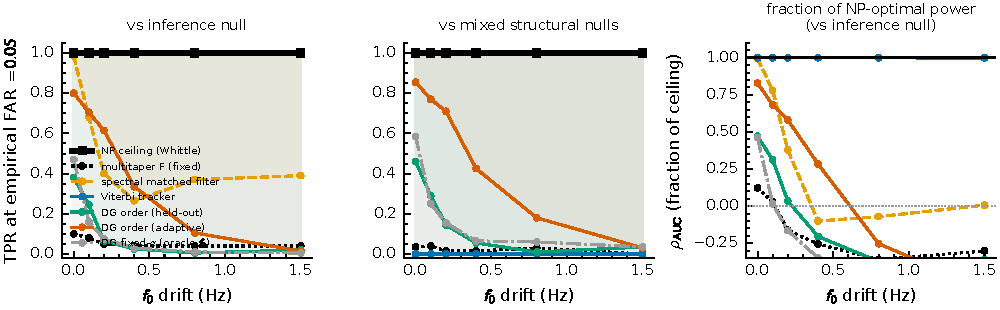
\includegraphics[width=\linewidth]{st1_np_ceiling}
	\caption{Corpus-free detectors as a fraction of the Whittle Neyman--Pearson
	ceiling versus cadence drift, against the inference null and the structural
	confusers. The ceiling is $1.0$ everywhere; the Viterbi tracker saturates it
	against the inference null, while only the tracked order family approaches it
	against the structural confusers. The gap that opens at high drift is the
	headroom above current detectors.}
	\label{fig:np_ceiling}
\end{figure*}

\section{Identifiability details}
\label{app:identifiability}

This appendix proves the results stated in \cref{subsec:identifiability} and
reports the numerical check that fixes their constants.

\paragraph{Proof of \cref{prop:noident}.}
A passive verifier observes only $P_{\mathrm{obs}}$, so its decision is a
measurable function $\phi$ of that trace and its rejection probability is
$\mathbb{E}_{K_h(w)}[\phi]$. If $K_{h_0}(w_0) = K_{h_1}(w_1)$ the two
expectations coincide for every $\phi$, so no test separates the pair, and no
post-processing of the trace can (data processing cannot create distinguishability
that the laws do not contain). The claim about restrictions follows by
contraposition: a non-vacuous guarantee must exclude the equivalent pairs, and
each listed lever excludes some of them. The amplitude degeneracy of
\cref{eq:device} shows the pairs are not exotic. The meter constrains only the
product $r(t)F(t)$, so a workload with a different operation rate and a
compensating energy cost per operation is already observationally equivalent, and
temporal structure --- not amplitude --- is what the trace identifies. The
near-constructive same-hardware case is the discarded-update decoy: forward,
backward, and optimiser kernels executed on the declared schedule with each
updated state discarded reproduces the compute/communication alternation, hence
the trace, without retaining a model. The converse direction is equally open to
the prover: genuine training can be run asynchronously, diluted among other
loads, or actively power-shaped, so the equivalence classes are populated from
both sides.

\paragraph{Proof of \cref{prop:rolloff}.}
Boundary $i$ nominally carries phase $2\pi i$; fractional period jitter perturbs
each boundary relative to its predecessor, so the \emph{residual} of the boundary
phase against a uniform clock accumulates independent increments and performs a
random walk with $\mathrm{Var}[\theta(t)] \approx D t$ and
$D \approx (2\pi)^2\sigma^2 f_0$. For a Brownian phase the periodic component's
autocorrelation decays as $\exp(-D|\tau|/2)$, so its spectrum is a Lorentzian
rather than a line, with half-width at half-maximum
$\gamma = D/4\pi = \pi\sigma^2 f_0$ in Hz. A record of length $T$ resolves
frequency only to $1/T$, so the coherent power a fixed-bin verifier collects is
the Lorentzian mass within a half-width $B = 1/2T$ of the centre,
\begin{equation}
	\frac{P_c(\sigma)}{P_c(0)}
	\;=\; \frac{2}{\pi}\arctan\!\left(\frac{B}{\gamma}\right)
	\;=\; \frac{2}{\pi}\arctan\!\left(\frac{1}{2\pi f_0 T \sigma^2}\right),
	\label{eq:arctan}
\end{equation}
whose small-argument form is $1/(\pi^2 f_0 T\sigma^2)$. Matching that tail to
$(1+\kappa\sigma^2)^{-1}$ gives
\begin{equation}
	\kappa \;=\; \pi^2 f_0 T,
	\label{eq:kappa}
\end{equation}
a parameter-free prediction rather than a fitted scale --- the width and bandwidth
conventions are fixed by the explicit calculation for the rectangular-bin, untapered
estimator used below, so no $O(1)$ factor is left free. The
Lorentzian of \cref{eq:rolloff} is not a pointwise approximation to
\cref{eq:arctan}: the two differ by up to $22\%$ near $\sigma = 0.02$, where the
arctan is still turning over, and agree to better than $1\%$ only for
$\sigma \gtrsim 0.2$. What matters is that using the Lorentzian as the fit model
does not bias the constant it returns --- fitting \cref{eq:rolloff} to
\cref{eq:arctan} across the $\sigma$ grid swept below recovers $\kappa = 2955$,
within $0.2\%$ of $\pi^2 f_0 T$.

\paragraph{Proof of \cref{prop:sigmastar}.}
Let $S$ be the fixed-bin statistic and consider the threshold tests
$\{S \geq c\}$. The advantage of the best such test is
$J = \sup_c \left(\Pr_{\mathrm{train}}[S \geq c] - \Pr_{\mathrm{null}}[S \geq
c]\right)$, the \emph{one-sided} Kolmogorov--Smirnov distance of the score laws
(one-sided because training traces score high, so only that direction is a
detection advantage; one-sided $\leq$ two-sided $\leq \mathrm{TV}$, so the
inequality we need still runs the right way). These are probabilities under the
two laws, so $J$ is a population quantity, and each $\{S \geq c\}$ is a
deterministic single-trace test that attains its own difference --- existence is
all \cref{def:covert} needs. Each such test is a measurable function of the trace,
so by data processing
$J \leq \mathrm{TV}(P_{\mathrm{train}},P_{\mathrm{null}})$. If
$J(\sigma) > \varepsilon$ then total variation exceeds $\varepsilon$ and the
attack is not $\varepsilon$-covert by \cref{def:covert}; equivalently,
$\varepsilon$-covertness requires $J(\sigma) \leq \varepsilon$. Empirically $J$
decreases in $\sigma$ over the swept range, so the requirement becomes a lower
bound $\sigma \geq \sigma^*(\varepsilon)$; we do not prove that monotonicity,
which would need a stochastic-ordering argument for the score laws rather than
merely the decay of the coherent power that drives them. Fitting the functional
form of \cref{eq:rolloff} to $J$, $J(\sigma) = J_0/(1+\kappa_J\sigma^2)$, and
inverting gives
\begin{equation}
	\sigma^*(\varepsilon)
	\;=\; \kappa_J^{-1/2}\,\sqrt{J_0/\varepsilon - 1},
	\label{eq:sigmastar}
\end{equation}
which grows like $\varepsilon^{-1/2}$ for small $\varepsilon$. That asymptotic
form is a property of the \emph{fitted} rolloff extrapolated beyond the swept
range, not a derived law, which is why \cref{prop:sigmastar} claims only that
$\sigma^*$ is positive and increases as $\varepsilon$ falls. Enlarging the
verifier class can only increase the attainable advantage at each $\sigma$, hence
only raise the class-indexed $\sigma^*_{\mathcal{C}}(\varepsilon) =
\inf\{\sigma : \sup_{\phi \in \mathcal{C}} J_\phi(\sigma) \leq \varepsilon\}$;
$\sigma^*$ above is that quantity for the singleton fixed-bin class.

Two points of bookkeeping. First, the rolloff constant $\kappa_J$ of the
\emph{advantage} is not the $\kappa$ of the \emph{coherent power} in
\cref{eq:rolloff}: the advantage saturates near one while any excess at $f_0$
remains separable from a line-free null, so it decays far more slowly. The two are
not interchangeable in either direction --- coherent power is not a detection
advantage at all, so it can never be substituted into \cref{eq:sigmastar},
whatever its rolloff. Second, $J$ is not interchangeable with the rank-based Gini
index $2\,\mathrm{AUC}-1$: the latter can exceed $J$, so it is not the advantage
of any single-trace test and cannot appear in \cref{eq:sigmastar}. Both are
reported in the summary artefact; only $J$ carries the bound.

\paragraph{Discussion of \cref{ass:cost}, and why it is an assumption.}
Hold the prover's total useful work fixed. Then a period is occupied either by
training work or by idling, and period jitter has two realisations. Padding with
idle time holds the real work per iteration fixed, so every period must be at
least as long as the compute it contains and the mean period inflates with
$\sigma$; throughput falls, and \cref{sec:frontier} measures the penalty at
$15$--$375\%$ over the swept range. Varying the real work per iteration avoids
idling and is measured at essentially zero throughput cost, but within
\cref{def:family} it cannot make the schedule aperiodic: the accumulated work is
an integer number of micro-steps, so the up-phase is quantised rather than
continuously tunable, and the exchange down-phase keeps its duration whatever that
count, leaving a component at the exchange cadence. Removing \emph{that} requires
either inserting idle time, which returns to the first realisation and its
throughput cost, or desynchronising the exchange, which alters the optimisation
actually performed and is therefore paid for in learning efficiency.

Two gaps stop this being a proof, and both matter.

The first is that the surviving component is not one the fixed-bin verifier can
use. \Cref{sec:frontier} measures the fixed tests under variable real work falling
to detection rate $0.26$ with area under the curve $0.44$ --- below chance --- and
the multitaper F-test at its floor. So the residual at the exchange cadence is
recovered only by the order-tracking class, which is precisely the class
\cref{prop:sigmastar} does \emph{not} instantiate. Read strictly, then, the
argument shows that a work-varying prover remains detectable \emph{by a tracker},
not that it must pay to become $\varepsilon$-covert against the fixed-bin verifier
whose $\sigma^*$ we computed. Closing that gap needs $\sigma^*$ for the tracking
class, which we do not have.

The second is that fixing total useful work is a real restriction. A prover free
to substitute useful \emph{non-training} work --- the additive-burial and dilution
families of \cref{subsec:adversary} --- can modulate the period while idling
neither the device nor the training job, and pays in neither training throughput
nor learning efficiency. Frequency scaling is a further route the two-realisation
dichotomy does not cover. So the disjunction holds over timing attacks at fixed
work, not over the adversary's full repertoire.

What the numerical check does support is the weaker comparative claim: at matched
total distortion, and for every $\sigma \geq 0.05$, the work-varying attack is
\emph{more}
detectable than idle-padded jitter, so substituting real-work variation does not
buy covertness for free relative to the priced attack --- it trades throughput
cost for detectability. That comparison is measured; the cost disjunction itself
is assumed, and \cref{ass:cost} is labelled accordingly.

\paragraph{Numerical check.}
\Cref{fig:lower_bound} tests every load-bearing step against the generator and
meter of \cref{sec:scenario} rather than an idealised channel. Training and
inference-null populations ($n=600$ per class, $f_0 = 1$~Hz, $T = 300$~s,
$f_s = 20$~Hz, seeded) are pushed through the full observation map and scored with
the fixed-bin statistic. The coherent power follows \cref{eq:rolloff} with
$R^2 = 0.95$ and a fitted $\kappa = 3068$ against the parameter-free
$\pi^2 f_0 T = 2961$ of \cref{eq:kappa}, with nothing fitted --- but that $4\%$
should be read as an order-of-magnitude agreement rather than a two-figure one.
The linearised fit weights each point by $\sigma^4$, so $81\%$ of its leverage
sits on the largest $\sigma$ swept, and there the generator realises a cadence CV
of $1.9$ against a nominal $0.5$: the mean period has drifted well off $f_0$ and
the fixed bin is no longer measuring line broadening alone. Restricting the fit to
the faithful regime $\sigma \leq 0.1$, where the realised CV tracks the nominal to
within about $13\%$, gives $\kappa = 2812$, or $5\%$ below the prediction. The
honest statement is agreement at the several-percent level from either end of the
sweep, which still separates $\pi^2 f_0 T$ from $\pi f_0 T$ by the factor of
$3.1$ that distinguishes them --- the strongest single confirmation of the physical
picture here.

The attained advantage requires more care, because it is estimated. Our plug-in
$\hat J$ maximises over thresholds on the same sample it evaluates, so it is
upward-biased; under $H_0$ at $n=600$ its fluctuation reaches $0.093$, and a
measured $\hat J$ below that carries no evidence of separation. Because the fit
linearises as $J_0/J-1$, which diverges as $J \to 0$, such points would otherwise
dominate it --- at the $n=80$ sizing we first used, two washed-out points carried
$97\%$ of the fit and $\kappa_J$ varied fourfold across seeds. We therefore
exclude points below the $H_0$ floor and report intervals. On the surviving window
$\sigma \in [0.05, 0.35]$ the advantage rolls off with $\kappa_J = 32$
($95\%$ bootstrap interval $[24, 40]$, $R^2 = 0.90$, $J_0 = 1.0$), giving
\begin{equation*}
	\sigma^*(0.5) = 0.18\ [0.16, 0.20], \qquad
	\sigma^*(0.2) = 0.36\ [0.32, 0.41],
\end{equation*}
and, by extrapolation beyond the swept range, $\sigma^*(0.1) = 0.53$ and
$\sigma^*(0.05) = 0.78$.

Two caveats bound how far these numbers travel. First, the generator realises the
nominal distortion only up to $\sigma \approx 0.2$: beyond it the reciprocal
Gaussian period draw and a clamp take over, and the measured cadence coefficient
of variation runs high ($1.2$ at $\sigma = 0.35$, $1.9$ at $\sigma = 0.5$),
as does $D$ against $(2\pi)^2\sigma^2 f_0$. Only $\sigma^*(0.5)$ falls inside that
faithful region; $\sigma^*(0.2)$ and everything beyond it do not, and the artefact
flags them. Second, the fit window reaches past $\sigma = 0.2$ by choice rather
than necessity: the five points at $\sigma \leq 0.2$ are unsaturated and do support
a fit, but the deep-rolloff point at $\sigma = 0.35$ carries most of the leverage
on $\kappa_J$. Restricting the fit to the faithful
region alone gives $\kappa_J = 22$ and hence larger thresholds, $\sigma^*(0.5) =
0.22$ and $\sigma^*(0.2) = 0.43$. The thresholds are therefore good to about
$20\%$, not to two significant figures, and the direction of that fit-window
uncertainty is towards \emph{more} required distortion, not less. Finally, the
work-varying series attains a higher advantage than period jitter at every
$\sigma \geq 0.05$, the two being indistinguishable within sampling error below
that, which is the comparison \cref{ass:cost} appeals to. Both arms set the
period-jitter scale explicitly, so this is a comparison at matched total
distortion.

\begin{figure*}[t]
	\centering
	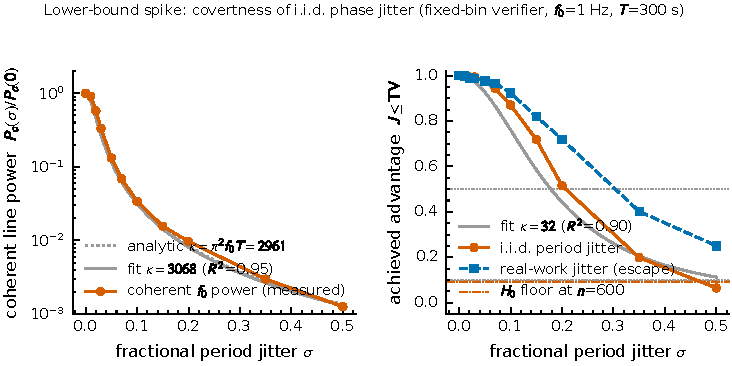
\includegraphics[width=\linewidth]{lower_bound_spike}
	\caption{Numerical check on the covertness cost bound, through the full
	generator and meter ($n=600$ per class). \textbf{Left:} coherent power at the
	nominal cadence against jitter scale. The fitted and the parameter-free
	analytic rolloffs of \cref{eq:rolloff,eq:kappa} are indistinguishable at this
	scale; the fitted constant agrees with the parameter-free prediction at the
	ten-percent level (see the numerical check). \textbf{Right:} the advantage attained by the
	fixed-bin threshold test, $J \leq \mathrm{TV}$, for idle-padded period jitter
	and for the near-free work-varying attack; dotted lines mark
	$\varepsilon \in \{0.1, 0.5\}$, whose crossings give
	$\sigma^*(\varepsilon)$ (the $\varepsilon = 0.1$ crossing lies beyond the
	swept range and is reached by extrapolation). The dash-dotted line is the
	$H_0$ fluctuation of the estimator: the $\sigma = 0.5$ point falls below it
	and is excluded from the advantage fit shown here (it is retained in the
	coherent-power fit on the left, which has no sampling floor of its own). For
	$\sigma \geq 0.05$ the work-varying attack is
	the more detectable of the two at matched distortion, the comparison
	\cref{ass:cost} appeals to; below that the two are indistinguishable within
	sampling error. Both arms set the period-jitter scale explicitly, so the
	distortion really is matched. The verifier
	here is fixed at the known cadence, not the order tracker of
	\cref{sec:structural}.}
	\label{fig:lower_bound}
\end{figure*}

\paragraph{From distortion to a price.}
The distortion thresholds can be read against the measured cost anchors of
\cref{sec:frontier}, which price the idle-padded realisation on the same nominal
$\sigma$ grid. Hiding from the fixed-bin verifier to $\varepsilon = 0.5$ needs
$\sigma^* = 0.18$, which falls between the measured levels $\sigma = 0.1$ and
$\sigma = 0.2$ and so between $32\%$ and $66\%$ throughput overhead; to
$\varepsilon = 0.2$ it needs $\sigma^* = 0.36$, between $159\%$ and $375\%$.
Given the roughly $20\%$ uncertainty on $\sigma^*$ established above, and the
scope limits of \cref{rem:boundscope,rem:costgap}, the robust
form of the statement is the order of magnitude rather than the bracket: driving a
fixed-bin verifier to $\varepsilon = 0.5$ costs \emph{tens of percent} of
throughput, and to $\varepsilon = 0.2$ costs \emph{of order $100\%$ or more}. Both
readings survive the fit-window sensitivity; the individual brackets do not, and
the $\varepsilon = 0.5$ one in particular moves up a level under the
faithful-region fit.

This is the sense in which the bound has a price, and \cref{fig:st2_cost_pareto}
is its empirical counterpart. Three things keep the two from being conflated. The
thresholds come from a fixed-bin verifier at the known cadence on $600$ traces per
class, whereas the frontier scores a five-detector bank on $200$. The pairing is
by nominal $\sigma$, but the two campaigns realise the same nominal setting
somewhat differently once past the faithful region --- cadence coefficient of
variation $0.50$ here against $0.84$ there at $\sigma = 0.35$ --- so the mapping is
exact only for $\sigma \lesssim 0.2$. And the frontier prices attacks against a
detector bank that includes the tracker, whose $\sigma^*$ we never computed. They
are read side by side, not on shared axes.

\paragraph{What the bound does not cover.}
The propositions above concern one attack family. Making the measured frontier a
statement about hiding in general would need one of two further arguments: that
the swept families span what a hiding adversary can do, or a bound of the kind
above for each of them. We have the second for i.i.d.\ period jitter and make no
claim of the first, so \cref{sec:frontier} should be read as a sample of the
attack space rather than its boundary. The choice of distributional distance is
also not settled. We use total variation, reached through an attained advantage;
Kullback--Leibler and Hellinger distances tensorise more conveniently over the
many-iteration product law and may give a tighter closed form, which we leave
open.

\end{document}
